\documentclass[twocolumn]{article}
\usepackage{a4}
\usepackage{graphicx}
\setlength{\textwidth}{160mm}
\setlength{\oddsidemargin}{0mm}
\setlength{\textheight}{230mm}
\setlength{\voffset}{0mm}
\setlength{\columnsep}{10mm}
\pagestyle{empty}

\begin{document}

\twocolumn[
\begin{center}

\includegraphics{honda-ftr.eps}

\vspace*{70pt}
{\LARGE
Details of EALib: What happened in EALib?}\\

\vspace*{10mm}

HRE-G / FTR Report 01 / 07\\

\vspace*{30mm}

August 8, 2001\\

\vspace*{30mm}

Tatsuya Okabe, Martina Hasenj\"{a}ger and Bernhard Sendhoff\\

Honda R\&D Europe (Deutschland) GmbH\\
Future Technology Research\\
Carl-Legien Strasse 30\\
D-63073 Offenbach / Main\\
Germany\\

\vspace*{30mm}

\end{center}

\noindent
Correspondence:

\noindent
tatsuya.okabe@hre-ftr.f.rd.honda.co.jp


]

\clearpage

\twocolumn[
\noindent
Report No. TO-2001-02

\noindent
Internal Report No. HRE-G/FTR 01/07

]

\clearpage

\twocolumn[

\begin{center}

{\bf {\LARGE Details of EALib: What happened in EALib?}}\\

\vspace*{10mm}

Tatsuya Okabe, Martina Hasenj\"{a}ger and Bernhard Sendhoff \\

\vspace*{10mm}

HONDA R\&D Europe ( Deutschland ) GmbH\\
Future Technology Research\\
Carl-Legien-Strasse 30 , 63073 Offenbach / Main , Germany\\

\vspace*{3mm}

{\bf tatsuya.okabe@hre-ftr.f.rd.honda.co.jp}\\

\end{center}

\vspace*{10mm}

\noindent
{\bf Abstract}\\
\normalsize
\noindent
The target of this report is to explain details of EALib \cite{EALib-int-1997}. 
Of course, there are a few manuals about EALib \cite{EALib-Man-2000}
\cite{EALib-Qui-2000} \cite{EALib-Ref-2000}. These manuals concentrate on
explaining how to use EALib, specially how to use EALib for evolution
strategies. However, in order to understand EALib completely or in
order to modify or update EALib, these manuals are not sufficient. 

\noindent
Our current target is to apply EMOO ( Evolutionary Multi-Objective
Optimization ) to EALib. Unfortunately, EALib was
designed for single objective. To modify EALib for EMOO, we had to
read the source
code. Thus, we will explain details of EALib from that experience in
this report.

\noindent
In EALib, about 1000 functions exist. Of course, we will not or can not
explain all functions. Thus we will concentrate on one topic: {\em What will
happen after declaring ``Population.h''}. However, if we select this
topic, about 400 functions already exist. Thus, regarding details of
functions, we will  explain the most important functions only.

\noindent
We will make this report for developers. Of course, it is our pleasure
that this report may help users to understand EALib.

\vspace*{5mm}

\noindent
{\bf Keywords}\\
\noindent
EALib, Evolutionary Computation

\vspace*{10mm}
]

%88888888888888888888888888888888888888888888888888888888888888888888
\section{Introduction}

\noindent
EALib is a C++ library for Evolutionary Algorithms, e.g. Genetic
Algorithms and Evolution Strategies. This library has been developed
by Ruhr University Bochum in 1996. We can get it from the
internet \cite{EALib-Address} as GPL2 ( GNU Public License Ver. 2 )
\cite{GPL2}. It can be run on UNIX, Linux and Windows.

\noindent
EALib was designed for Evolutionary Algorithms. Furthermore, there
are many excellent classes in it, e.g. random number generators,
principal component analysis, array, linear algebra and so on. In our
division, we are using EALib for our research to reduce the time of
programming, to shorten the code and to decrease the possibility of 
bugs. 

\noindent
EALib has about 60 classes and 1000 functions in Version
1.5. But EALib was well structured according to some rules. Thus, it
is easier to understand them than expected.

\noindent
In this report, we will explain more details of EALib than existing
manuals to help developers. We will explain one topic in each
section, e.g. Header files, Classes, Functions and details of
important functions.

%88888888888888888888888888888888888888888888888888888888888888888888
\section{Header Files}

\noindent
In order to use EALib, we have to include the command {\em \#include
``Population.h''}. Of course, in the header file {\em Population.h},
other header files will be included and they will let others be
included. This flow is shown in Figure \ref{Header}.

\noindent
At first, {\em Population.h} includes the next header file {\em
Individual.h}. Second, {\em Individual.h} includes the third header
file {\em ChromosomeT.h} and so on. Finally, we reach {\em RNG.h}. 

\noindent
For a developer, it is necessary to see these header files to
understand what happens in them. The following Table \ref{Header} will
explain where we can see them because they exist in different
folders. In this table, '*' means the folder where you installed EALib.

\noindent
As mentioned before, EALib has many other classes. However,
other classes will not be included without special
declarations. Regarding, other usefull classes, please see Appendix
A.


\begin{figure}[h]
\begin{center}
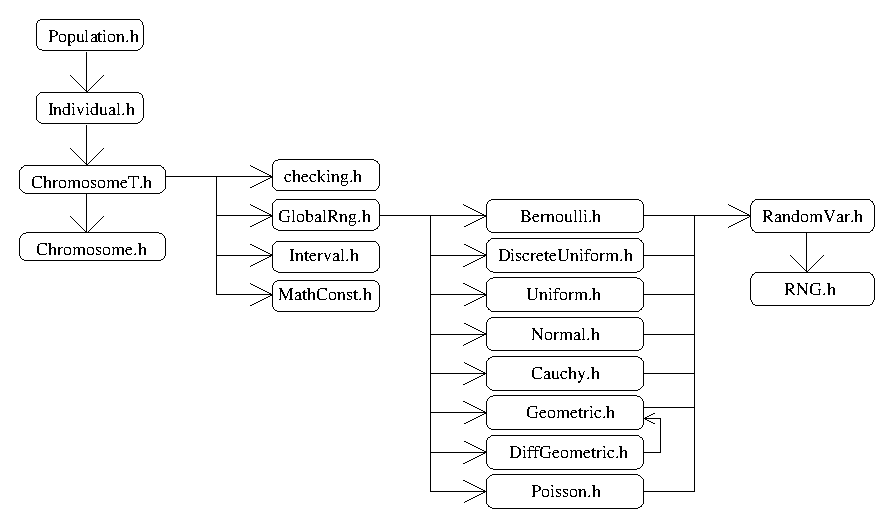
\includegraphics[width=7.5cm]{EALib-1.eps}\\
\caption{Header files}
\label{Header}
\end{center}
\end{figure}


\begin{table}[h]
\begin{center}
\caption{Header files}
\label{Header-Table}
{\scriptsize
\begin{tabular}{|l|l|}\hline
Header file       & Folder                            \\\hline\hline
Population.h      & */Shark-1.0/EALib/include/        \\\hline
Individual.h      & */Shark-1.0/EALib/include/        \\\hline
ChromosomeT.h     & */Shark-1.0/EALib/include/        \\\hline
Chromosome.h      & */Shark-1.0/EALib/include/        \\\hline
checking.h        & */Shark-1.0/Tools/Basics/include/ \\\hline
GlobalRng.h       & */Shark-1.0/Tools/Rng/include/    \\\hline
Interval.h        & */Shark-1.0/Tools/Basics/include/ \\\hline
MathConst.h       & */Shark-1.0/Tools/Math/include/   \\\hline
Bernoulli.h       & */Shark-1.0/Tools/Rng/include/    \\\hline
DiscreteUniform.h & */Shark-1.0/Tools/Rng/include/    \\\hline
Uniform.h         & */Shark-1.0/Tools/Rng/include/    \\\hline
Normal.h          & */Shark-1.0/Tools/Rng/include/    \\\hline
Cauchy.h          & */Shark-1.0/Tools/Rng/include/    \\\hline
Geometric.h       & */Shark-1.0/Tools/Rng/include/    \\\hline
DiffGeometric.h   & */Shark-1.0/Tools/Rng/include/    \\\hline
Poisson.h         & */Shark-1.0/Tools/Rng/include/    \\\hline
RandomVar.h       & */Shark-1.0/Tools/Rng/include/    \\\hline
RNG.h             & */Shark-1.0/Tools/Rng/include/    \\\hline
\end{tabular}
}
\end{center}
\end{table}

%88888888888888888888888888888888888888888888888888888888888888888888
\section{Classes}

\noindent
As mentioned, EALib has many classes. But, it is well structured. In
this section, we will explain the classes in EALib and their
structure. Additionally, the data structure and internal variables in each
class will be explained.

\noindent
In C++, the definition of a class is done in the corresponding
header file. The next Table \ref{IncludeClass} will show the existing
classes in each header file. 

\noindent
Regarding other classes, please see Appendix B.

\begin{table}[h]
\begin{center}
\caption{Including classes}
\label{IncludeClass}
{\footnotesize
\begin{tabular}{|l|l|}\hline
File name         & Including classes             \\\hline\hline 
Population.h      & $Class \ Population         $ \\\hline
Individual.h      & $Class \ Individual         $ \\\hline
ChromosomeT.h     & $Class \ ChromosomeT\_base  $ \\
                  & $Class \ ChromosomeT        $ \\
                  & $Class \ ChromosomeT\_num   $ \\
                  & $Class \ ChromosomeT<double>$ \\
                  & $Class \ DerandomConst      $ \\
                  & $Class \ ChromosomeT<char>  $ \\
                  & $Class \ ChromosomeT<int>   $ \\
                  & $Class \ ChromosomeT<bool>  $ \\\hline
Chromosome.h      & $Class \ Chromosome         $ \\\hline
checking.h        & $(nothing)                  $ \\\hline
GlobalRng.h       & $Class \ Rng                $ \\\hline
Interval.h        & $Class \ Interval           $ \\\hline
MathConst.h       & $(nothing)                  $ \\\hline
Bernoulli.h       & $Class \ Bernoulli          $ \\\hline
DiscreteUniform.h & $Class \ DiscreteUniform    $ \\\hline
Uniform.h         & $Class \ Uniform            $ \\\hline
Normal.h          & $Class \ Normal             $ \\\hline
Cauchy.h          & $Class \ Cauchy             $ \\\hline
Geometric.h       & $Class \ Geometric          $ \\\hline
DiffGeometric.h   & $Class \ DiffGeometric      $ \\\hline      
Poisson.h         & $Class \ Poisson            $ \\\hline
RandomVar.h       & $Class \ RandomVar          $ \\\hline
RNG.h             & $Class \ RNG                $ \\\hline
\end{tabular}
}
\end{center}
\end{table}

\noindent
EALib was well structured for Evolutionary Computation. In order to
develop a program for Evolutionary Computation, we will use the classes {\em
Population}, {\em Individual} and {\em Chromosome}. Furthermore, EALib 
offers some classes for {\em Chromosome} according to the type of 
alleles. 

\noindent
To explain the well-structured classes, at first we will show the flow of
Evolutionary Computation using Figure \ref{EC}.

\begin{figure}[h]
\begin{center}
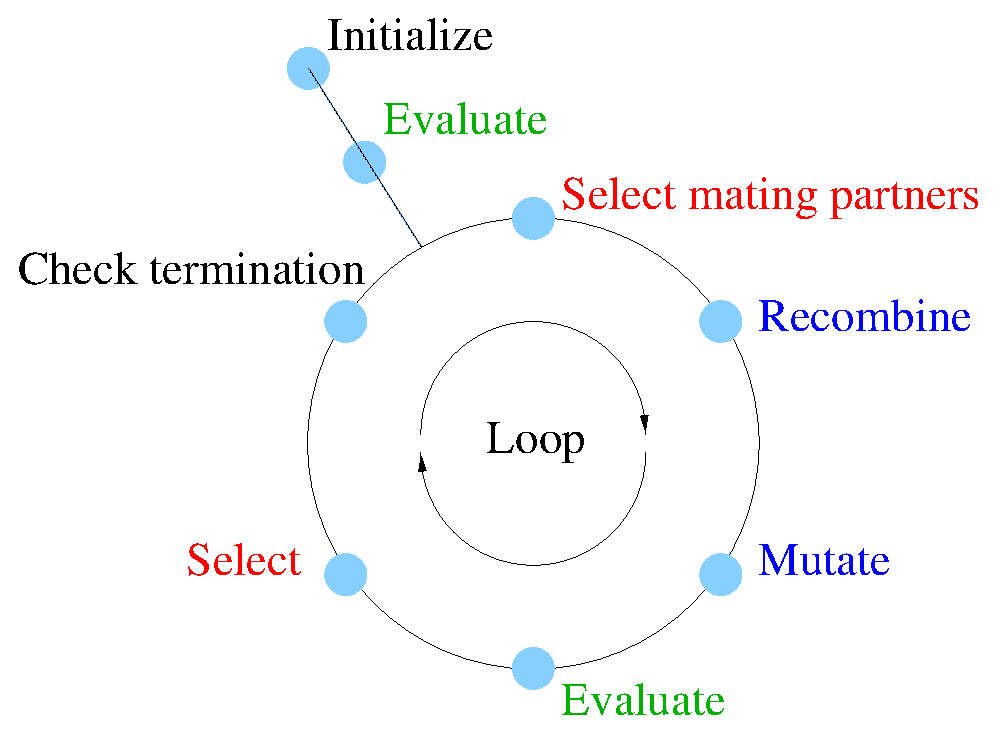
\includegraphics[width=7cm]{EvolutionaryComputation.eps}
\caption{The flow of Evolutionary Computation}
\label{EC}
\end{center}
\end{figure}

\noindent
In this flow, several steps exist, e.g. Initialize, Evaluate etc.

\noindent
To implement {\em Select mating partners} and {\em Select}, we have to see all
individuals. Thus {\em Select mating partners} and {\em Select} will
be done by class
Population. Regarding {\em Evaluate}, we have to see one individual
and all alleles. For implementation of {\em Evaluate}, this will be
done by class Individual. Finally, to do {\em Recombinate} and {\em
Mutate}, we have to see in the chromosome. So, these will be done by class Chromosome.

\noindent
In EALib, the functions were divided into classes according to
the former explanation. This division helps us to easily understand
EALib. Class {\em Population} has functions for treating
individuals, class {\em Individual} for treating chromosomes and
class {\em Chromosome} for treating alleles.

\noindent
Figure \ref{RoleOfClass} shows the role of each class and internal
variables. The explanation for internal variables will be given later.

\vspace*{5mm}

\begin{figure}[h]
\begin{center}
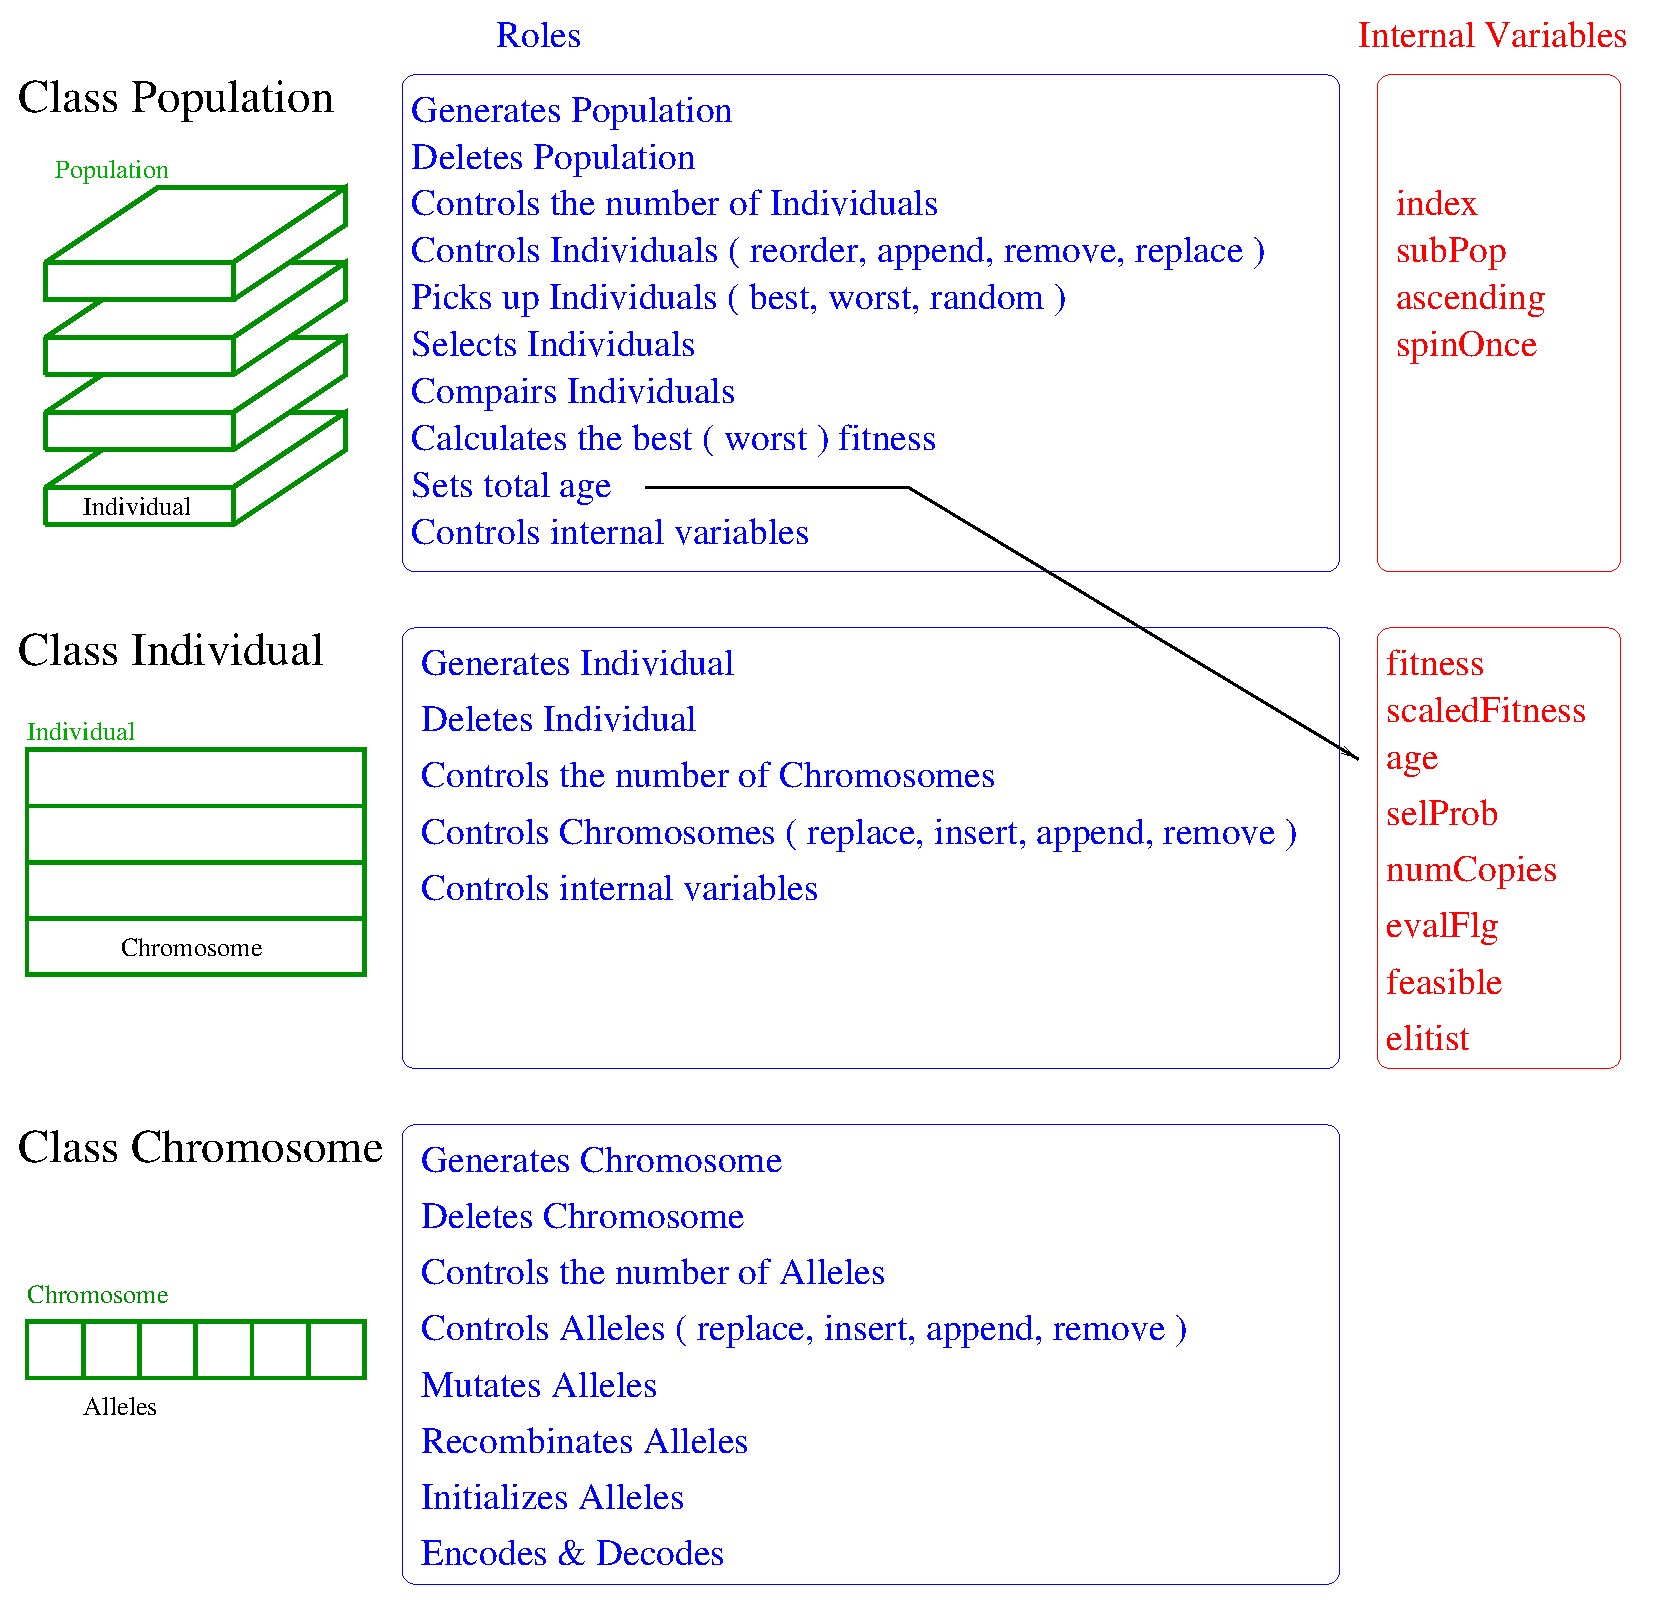
\includegraphics[width=8cm]{class-relationship.eps}
\caption{The role of each class}
\label{RoleOfClass}
\end{center}
\end{figure}

\noindent
From Figure \ref{RoleOfClass}, perhaps you can understand where functions belong
to and why functions belong to that class.

\noindent
Now, we would like to explain the structure of data. Class {\em
Population} has a vector to store the starting addresses of class {\em
Individual} and class {\em Individual} has another vector to store those 
of class {\em Chromosome}. And class {\em Chromosome} has a vetctor
for alleles. Each vector will be generated automatically in the
constructor of each class.

\noindent
Class {\em Population} and {\em Individual} have internal
variables we showed in Figure \ref{RoleOfClass}. These variables
mean the following:

{\small 
\begin{description}
\item[index :] the index of the individual with the best fitness.
\item[subPop :] denotes whether the population is a subpopulation or
not.
\item[ascending :] the individuals in the population are sorted
according to their fitness values. This variable corresponds to {\em
Maximum Problem} or {\em Minimum Problem}.
\item[spinOnce :] indicates whether the roulette wheel will spin only
one time or several times.
\item[fitness :] result of the evaluation of an individual.
\item[scaledFitness :] result of the fitness scaled by scaling
function.
\item[age :] the age of the individual.
\item[selProb :] the selection probability of the individual.
\item[numCopies :] denotes the number of reproductions of the
individual during the last selection.
\item[evalFlg :] denotes whether the fitness of the individual must
be evaluated or not.
\item[feasible :] denotes whether the current individual is a
possible solution for the optimization problem or not.
\item[elitist :] denotes whether the individual was selected as an
elitist during the last selection or not.
\end{description}
}

%88888888888888888888888888888888888888888888888888888888888888888888
\section{Functions and details of important functions}

\noindent
We will show functions in EALib. However, there are about 1000
functions in EALIb.

\noindent
The next table shows the number of functions which you can use after
including ``{\em Population.h}''. The total number is about 400.

\noindent
Additionally, about 150 functions exist as global functions.

\noindent
Regarding other functions that belong to other classes, please see
Appendix C.

\noindent
We counted the number of public functions, private functions,
protected functions and other functions, e.g. virtual functions,
friend functions and inline functions, respectively.

\begin{table}[h]
\begin{center}
\caption{The number of functions}
\label{NoFunctions}
{\scriptsize
\begin{tabular}{|l|l|l|l|l|l|l|}\hline
Name of Class              & Public & Private & Protect & Others  \\\hline\hline
Population                 &     72 &      11 &       0 &       3 \\\hline
Individual                 &     39 &       0 &       0 &       3 \\\hline
ChromosomeT                &     46 &       0 &       2 &       0 \\
\hspace*{2mm} \_base       &        &         &         &         \\\hline
ChromosomeT                &      4 &       0 &       4 &       0 \\\hline
ChromosomeT                &     16 &       2 &       0 &       0 \\
\hspace*{2mm} \_num        &        &         &         &         \\\hline
ChromosomeT                &     60 &       0 &       4 &       0 \\
\hspace*{2mm} $<$double$>$ &        &         &         &         \\\hline
DerandomConst              &      3 &       0 &       0 &       0 \\\hline
ChromosomeT                &      4 &       0 &       4 &       0 \\
\hspace*{2mm} $<$char$>$   &        &         &         &         \\\hline 
ChromosomeT                &      8 &       0 &       4 &       0 \\
\hspace*{2mm} $<$int$>$    &        &         &         &         \\\hline 
ChromosomeT                &     15 &       0 &       4 &       0 \\
\hspace*{2mm} $<$bool$>$   &        &         &         &         \\\hline 
Chromosome                 &      1 &       0 &       0 &      41 \\\hline
Rng                        &      1 &       0 &       0 &       0 \\\hline
Interval                   &      6 &       0 &       0 &       0 \\\hline
Bernoulli                  &      7 &       0 &       0 &       0 \\\hline
DiscreteUniform            &      9 &       0 &       0 &       0 \\\hline
Uniform                    &      9 &       0 &       0 &       0 \\\hline
Normal                     &     10 &       0 &       0 &       0 \\\hline
Cauchy                     &      4 &       0 &       0 &       0 \\\hline
Geometric                  &      7 &       0 &       0 &       0 \\\hline
DiffGeometric              &      5 &       0 &       0 &       0 \\\hline
Poisson                    &      7 &       0 &       0 &       0 \\\hline
RandomVar                  &      2 &       0 &       1 &       6 \\\hline
RNG                        &      7 &       0 &       0 &       1 \\\hline
\end{tabular}
}
\end{center}
\end{table}

\noindent
Of course, we will not and can not introduce all functions. We will only
introduce details of some important functions. 

\noindent
To explain all functions is time-consuming and has no effect for users
and developers because many functions are very similar. 

\noindent
After you read this section, probably you can imagine other functions
that we will not explain here. We hope that the following explanation
helps you to easily understand other functions.

\noindent
At first, we selected the most important functions which users often
use. Our selection will be shown in the table \ref{MostImportant}.

\noindent
The first function is for generating a new population. The second is
for inserting an individual in an existing population. The third and
the forth are for selection. The fifth is for generating a new
individual. The sixth is for crossover. The seventh and the eighth are
for mutation. The last one is for recombination.

\noindent
Probably, we included all important genetic operators, e.g. mutation,
crossover, recombination and selection, and important constructors
which generate a new population and a new individual.

\noindent
If some important functions or other functions which you are
interested in are missing, please inform us. In the next version of
this paper, we will update them with pleasure.

\begin{table}[h]
\begin{center}
\caption{Most important functions}
\label{MostImportant}
{\scriptsize
\begin{tabular}{|l|l|}\hline
Function                                        & Class                       \\\hline \hline
Population( unsigned,                           & Population                  \\
\hspace*{2mm} const Chromosome\& )              &                             \\\hline
void insert( unsigned i,                        & Population                  \\
\hspace*{2mm} const Individual\& ind )          &                             \\\hline         
void selectMuLambda(                            & Population                  \\
\hspace*{2mm} Population\& parents,             &                             \\
\hspace*{2mm} unsigned nelitists = 0 )          &                             \\\hline
void selectLinearRanking(                       & Population                  \\
\hspace*{2mm} Population\& parents,             &                             \\   
\hspace*{2mm} double etaMax = 1.1,              &                             \\
\hspace*{2mm} unsigned nelitists = 0 )          &                             \\\hline 
Individual( const Chromosome\&,                 & Individual                  \\
\hspace*{2mm} const Chromosome\& )              &                             \\\hline      
void crossoverUniform(                          & ChromosomlT                 \\
\hspace*{2mm} const Chromosome\& dadChrom,      & \hspace{2mm} \_base         \\ 
\hspace*{2mm} const Chromosome\& momChrom,      &                             \\
\hspace*{2mm} const Chromosome\& posChrom )     &                             \\\hline
void mutateUniform(                             & ChromosomlT                 \\
\hspace*{2mm} const Chromosome\& min,           & \hspace{2mm} \_num          \\
\hspace*{2mm} const Chromosome\& max,           &                             \\
\hspace*{2mm} const Chromosome\& p,             &                             \\
\hspace*{2mm} bool cycle = false )              &                             \\\hline  
void mutateNormal(                              & ChromosomlT                 \\
\hspace*{2mm} const ChromosomeT$<$ double $>$\& & \hspace{2mm} $<$ double $>$ \\       
\hspace*{2mm} stddev, bool = false )            &                             \\\hline 
void recombineIntermediate(                     & ChromosomlT                 \\
\hspace*{2mm} Chromosome\& )                    & \hspace{2mm} $<$ double $>$ \\\hline
\end{tabular}
}
\end{center}
\end{table}


\subsection{Generate a new population}

\noindent
In this section, we will explain the following function in {\em Class
Population}.

\begin{center}
Population( unsigned n, const Chromosome\& chrom0 )
\end{center}

\noindent
The function prototype of this function was written in {\em
Population.h} and the source code was written in
{\em Population.cpp}. The function prototype and source code are given
in
Table \ref{FP1} and Table \ref{SC1}.

\begin{table}[h]
\begin{center}
\caption{The function prototype}
\label{FP1}
{\scriptsize
\begin{tabular}{|l|}\hline
\hspace*{7cm} \\
class Population : private vector$<$ Individual * $>$\\
\{\\
\hspace*{4mm} public:\\
\hspace*{8mm} Population( unsigned, const Individual\& );\\
\}\\
\\\hline
\end{tabular}
}
\end{center}
\end{table}

\begin{table}[h]
\begin{center}
\caption{The source code}
\label{SC1}
{\scriptsize
\begin{tabular}{|l|}\hline
\hspace*{7cm}\\
Population::Population( unsigned n,  const \\
\hspace*{4mm} Chromosome\& chrom0 ): vector$<$ Individual * $>$( n )\\
\{\\
\hspace*{4mm} for( unsigned i = size( ); i- -; )\\
\hspace*{8mm} *( begin( ) + i ) = new Individual( chrom0 );\\
\hspace*{4mm} subPop = false;\\
\hspace*{4mm} ascending = false;\\
\hspace*{4mm} spinOnce  = true;\\
\}\\
\\\hline
\end{tabular}
}
\end{center}
\end{table}

\noindent
This function generates a new population which has {\em n}
individuals. And all individuals are formed by cloning chromosome {\em
chrom0}. The image of this function is Figure \ref{GeneratePop}.

\begin{figure}[h]
\begin{center}
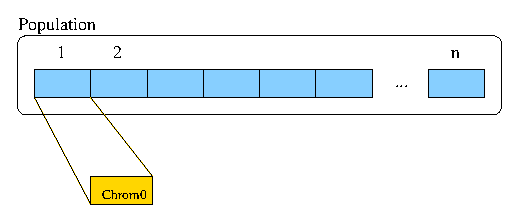
\includegraphics[width=5cm]{004-4-1-population5.eps}
\caption{Generates a new population}
\label{GeneratePop}
\end{center}
\end{figure}

\noindent
Now, let's see the source code. The function {\em Individual( chrom0
)} is for generating the chromosome which is formed by cloning
chromosome {\em chrom0}. Using variable {\em i}, ``{\em *(begin( ) + i)
= new Individual( chrom 0 )}'' will occur {\em n} times. ``{\em begin(
)}'' means the pointer which indicates the starting address of this
population. The variable {\em i} starts from {\em n-1} and ends at
{\em 0}. Thus, new chromosomes will be put into the addresses from ``{\em
begin( ) + (n-1)}'' to ``{\em begin( )}''.

\noindent
At the same time, internal variables, {\em subPop}, {\em ascending}
and {\em spinOnce}, will be set to default values.

{\small
\noindent
subPop = false ( This population is not a sub population. )

\noindent
ascending = false ( The problem is a ``Maximize'' problem. )

\noindent
spinOnce = true ( The roulette wheel will spin only one time. )
}

\subsection{Insert Individual}

\noindent
In this section, we will explain the following function in {\em Class
Population}. 

\begin{center}
void insert( unsigned i, const Individual\& ind )
\end{center}

\noindent
The function prototype of this function was written in {\em
Population.h} and the source code was written in {\em
Population.cpp}. The function prototype and source code are given in Table
\ref{FP2} and Table \ref{SC2}.

\begin{table}[h]
\begin{center}
\caption{The function prototype}
\label{FP2}
{\scriptsize
\begin{tabular}{|l|}\hline
\hspace*{7cm}\\
class Population : private vector$<$ Individual * $>$\\
\{\\
\hspace*{4mm} public:\\
\hspace*{8mm} void insert( unsigned i, const Individual\& ind );\\
\}\\
\hspace*{7cm}\\\hline
\end{tabular}
}
\end{center}
\end{table}

\begin{table}[h]
\begin{center}
\caption{The source code}
\label{SC2}
{\scriptsize
\begin{tabular}{|l|}\hline
\hspace*{7cm}\\
void Population::insert( unsigned i, \\
\hspace*{4mm} const Individual\& ind )\\
\{\\
\hspace*{4mm} RANGE\_CHECK( i $<$= size( ) )\\
\hspace*{4mm} vector$<$ Individual * $>$::insert( begin( ) + i, \\
\hspace*{8mm} new Individual( ind ) );\\
\}\\
\hspace*{7cm}\\\hline
\end{tabular}
}
\end{center}
\end{table}

\noindent
This function inserts an individual {\em ind} at the position {\em
i}. The image of this function is given in Figure \ref{InsertInd}.

\begin{figure}[h]
\begin{center}
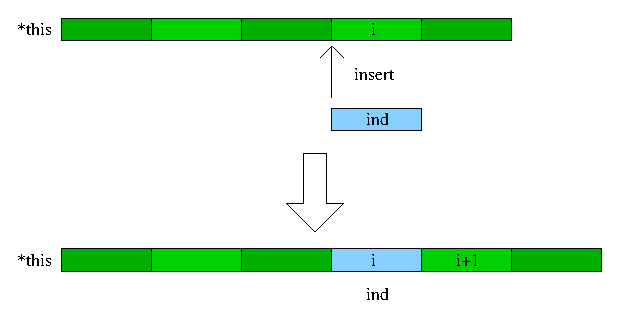
\includegraphics[width=5cm]{004-4-1-insert1.eps}
\caption{Inserts a Individual}
\label{InsertInd}
\end{center}
\end{figure}

\noindent
Let's see the source code. This function is very easy and has 2
commands only. At first, in ``{\em RANGE\_CHECK( i $<$= size( ) )}'',
variable {\em i} will be checked because variable {\em i} must be
between 0 and the number of Individuals - 1. In next command ``{\em
vector$<$ Individual * $>$::insert( begin( ) + i, new Individual( ind
) );}'', using $<$ vector $>$ containers, individual {\em ind} will be
inserted.

\subsection{Select Individuals 1}

\noindent
In this section, we will explain the following function in {\em Class
Population}. 

\begin{center}
void selectMuLambda( Population\& parents, unsigned nelitists = 0 )
\end{center}

\noindent
The function prototype of this function was written in {\em
Population.h} and the source code was written in {\em
Population.cpp}. The function prototype and source code are given in Table
\ref{FP3} and Table \ref{SC3}.

\begin{table}[h]
\begin{center}
\caption{The function prototype}
\label{FP3}
{\scriptsize
\begin{tabular}{|l|}\hline
\hspace*{7cm}\\
class Population : private vector$<$ Individual * $>$\\
\{\\
\hspace*{4mm} public:\\
\hspace*{8mm} void selectMuLambda( Population\& parents, \\
\hspace*{12mm} unsigned nelitists = 0 );\\
\}\\
\hspace*{7cm}\\\hline
\end{tabular}
}
\end{center} 
\end{table}

\begin{table}[h]
\begin{center}
\caption{The source code}
\label{SC3}
{\scriptsize
\begin{tabular}{|l|}\hline
\hspace*{7cm}\\
void Population::selectMuLambda( Population\& parents, \\
\hspace*{4mm} unsigned numElitists )\\
\{\\
\hspace*{4mm} unsigned i, j;\\
\hspace*{4mm} //\\
\hspace*{4mm} // clear number of copies and select elitists\\
\hspace*{4mm} //\\
\hspace*{4mm} parents.selectInit( );\\
\hspace*{4mm} selectElitists( parents, numElitists );\\
\hspace*{4mm} //\\
\hspace*{4mm} // sort parents (only pointers)\\
\hspace*{4mm} //\\
\hspace*{4mm} vector$<$ Individual * $>$ indvec( parents );\\
\hspace*{4mm} sortIndividuals( indvec );\\
\hspace*{4mm} for( i = numElitists, j = 0; i $<$ size( ) \&\& \\
\hspace*{8mm} j $<$ indvec.size( ); j++ ) \{\\
\hspace*{8mm} if( $!$ indvec[ j ]-$>$elitist ) \{\\
\hspace*{12mm} indvec[ j ]-$>$numCopies++;\\
\hspace*{12mm} ( *this )[ i++ ] = *indvec[ j ];\\
\hspace*{8mm} \}\\
\hspace*{4mm} \}\\
\hspace*{4mm} //\\
\hspace*{4mm} // fill remaining slots with the last/worst individual\\
\hspace*{4mm} //\\
\hspace*{4mm} while( i $<$ size( ) ) \{\\
\hspace*{8mm} indvec[ j-1 ]-$>$numCopies++;\\
\hspace*{8mm} ( *this )[ i++ ] = *indvec[ j-1 ];\\
\hspace*{4mm} \}\\
\}\\
\hspace*{7cm}\\\hline
\end{tabular}
}
\end{center}
\end{table}

\noindent
This function selects individuals by deterministic selection using ($\mu$,$\lambda$) or
($\mu$+$\lambda$) strategies. If {\em numElitists} = 0, this
corresponds to ($\mu$,$\lambda$) selection and if {\em numElitists} $>$ 0,
this corresponds ($\mu$+$\lambda$) selection.

\noindent
Let's see the source code.

\vspace*{2mm}

\noindent
\underline{parents.selectInit( );}

\noindent
This function sets internal variables in {\em parents} using default values.

\begin{equation}
numCopies = 0
\end{equation}
\begin{equation}
elitist = false
\end{equation}

\vspace*{2mm}

\noindent
\underline{selectElitists( parents, numElitists );}

\noindent
This function picks up {\em numElitists} individuals as elitist(s) from
(*this) \& {\em parents}. And also sets or calculates internal variables {\em
selProb}, {\em numCopies} and {\em elitist}. In this process, {\em
numElitists} individuals will be stored in (*this)[i] ( i=0,.....,numElitists-1 ).

\begin{equation}
selProb -= min( selProb, 1/size( ) );
\end{equation}
\begin{equation}
numCopies ++;
\end{equation}
\begin{equation}
elitist = true;
\end{equation}

\noindent
The flow of this function is shown in Figure \ref{SelectElitist}.

\begin{figure}[h]
\begin{center}
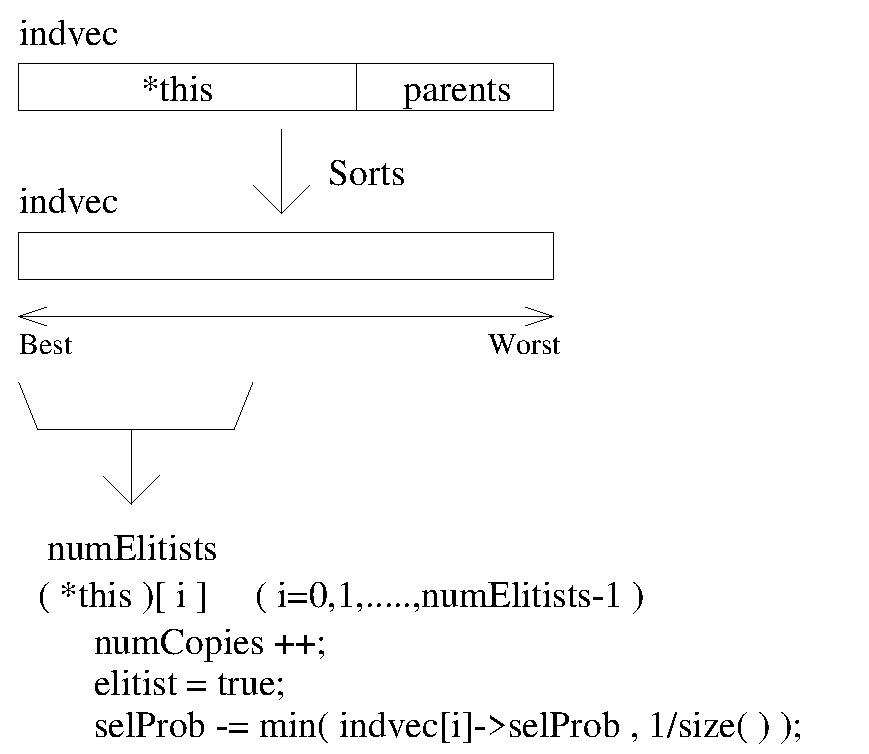
\includegraphics[width = 5cm]{selectElitists.eps}
\caption{Selects Elitists}
\label{SelectElitist}
\end{center}
\end{figure}

\vspace*{2mm}

\noindent
\underline{vector$<$ Individual * $>$ indvec( parents );}

\noindent
This command generates vector$<$ Individual * $>$ from {\em parents}.

\vspace*{2mm}

\noindent
\underline{sortIndividuals( indvec );}

\noindent
This command sorts individuals {\em indvec} according to {\em
ascending-flag}. In this command, ``std::sort'' will be used. After
this command, indvec[0] is the best individual and
indvec[indvec.size( )-1] is the worst individual.

\vspace*{2mm}

\noindent
\underline{for( i = numElitists, j = 0 ; i $<$ size( ) \&\&} \\
\underline{ j $<$ indvec.size( ) ; j++ )\{ ... \}} 

\noindent
This group of several commands picks up the remaining individuals from {\em
parents} and also sets the internal variable {\em numCopies}. These
individuals will be stored in (*this)[i] ( i = numElitists , ..... , size(
) - 1 or numElitists + indvec.size( ) ).

\begin{equation}
numCopies++;
\end{equation}

\noindent
We show the image of these commands in Figure
\ref{SelectOtherIndividuals}.

\begin{figure}[h]
\begin{center}
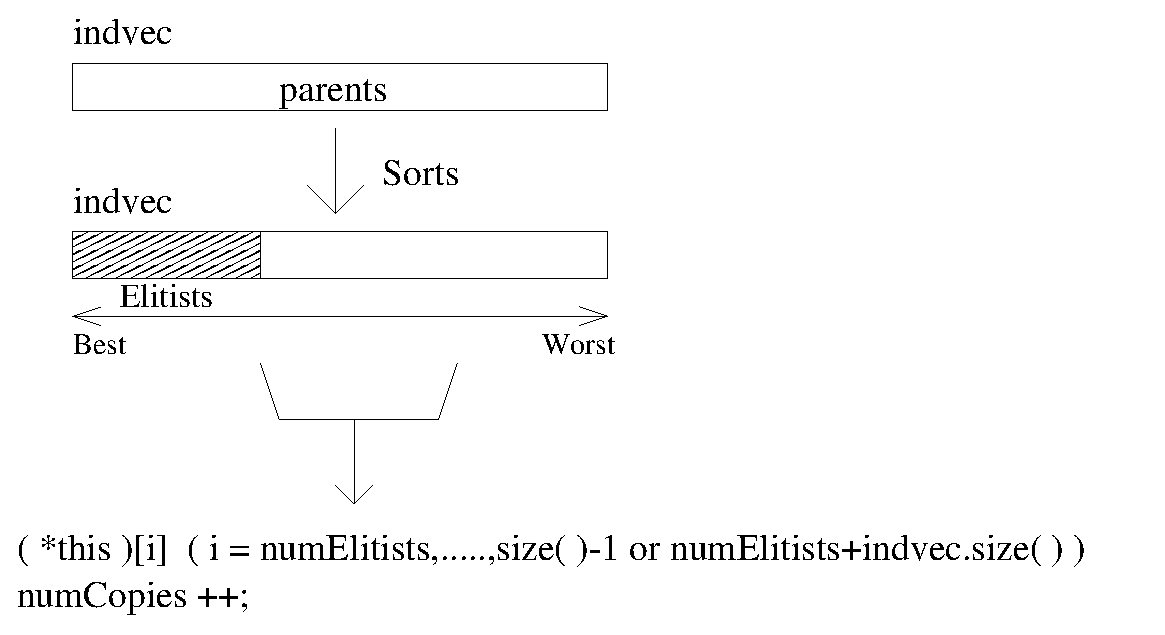
\includegraphics[width = 7.5cm]{selectMuLambda2.eps}
\caption{Selects other individuals}
\label{SelectOtherIndividuals}
\end{center}
\end{figure}

\noindent
\underline{while( i $<$ size( ) )\{ ... \}}

\noindent
If the number of individuals we picked up is not enough, this part
picks up the remaining individuals to satisfy the number. Those individuals are
made from the worst individual.

\subsection{Select Individual 2}

\noindent
In this section, we will explain the following function in {\em Class
Population}. 

\begin{center}
void selectLinearRanking( Population\& parents, double etaMax = 1.1,
unsigned nelitists = 0 )
\end{center}

\noindent
The function prototype of this function was written in {\em
Population.h} and the source code was written in {\em
Population.cpp}. The function prototype and source code are given in Table
\ref{FP4} and Table \ref{SC4}.

\begin{table}[h]
\begin{center}
\caption{The function prototype}
\label{FP4}
{\scriptsize
\begin{tabular}{|l|}\hline
\hspace*{7cm}\\
class Population : private vector$<$ Individual * $>$\\
\{\\
\hspace*{4mm} public:\\
\hspace*{8mm} void selectLinearRanking( Population\& parents, \\
\hspace*{12mm} double etaMax = 1.1,\\
\hspace*{12mm} unsigned nelitists = 0 );\\
\}\\ 
\hspace*{7cm}\\\hline
\end{tabular}
}
\end{center}
\end{table}

\begin{table}[h]
\begin{center}
\caption{The source code}
\label{SC4}
{\scriptsize
\begin{tabular}{|l|}\hline
\hspace*{7cm}\\
void Population::selectLinearRanking( Population\& \\
\hspace*{4mm} parents, double etaMax,\\
\hspace*{4mm} unsigned numElitists )\\
\{\\
\hspace*{4mm} if( size( ) == 0 $\mid \mid$ parents.size( ) == 0 )\\
\hspace*{8mm} return;\\
\hspace*{4mm} else if( parents.size( ) == 1 )\\
\hspace*{8mm} //\\
\hspace*{8mm} // if the parent population has only one \\
\hspace*{8mm} // individual it receives selection \\
\hspace*{8mm} // probability 1
\hspace*{8mm} //\\
\hspace*{8mm} parents[ 0 ].selProb = 1;\\
\hspace*{4mm} else \{\\
\hspace*{8mm} //\\
\hspace*{8mm} // sort parents (only pointers)\\
\hspace*{8mm} //\\
\hspace*{8mm} vector$<$ Individual * $>$ indvec( parents );\\
\hspace*{8mm} sortIndividuals( indvec );\\
\hspace*{8mm} //\\
\hspace*{8mm} // selection probabilities\\
\hspace*{8mm} //\\
\hspace*{8mm} double a = 2 * ( etaMax - 1 ) / ( indvec.size( ) \\
\hspace*{12mm}  - 1 );\\
\hspace*{8mm} for( unsigned i = 0; i $<$ indvec.size( ); i++ )\\
\hspace*{12mm} indvec[ i ]-$>$selProb = ( etaMax - a * i ) / \\
\hspace*{16mm} indvec.size( );\\
\hspace*{4mm} \}\\
\hspace*{4mm} //\\
\hspace*{4mm} // clear number of copies and select elitists\\
\hspace*{4mm} //\\
\hspace*{4mm} parents.selectInit( );\\
\hspace*{4mm} selectElitists( parents, numElitists );\\
\hspace*{4mm} //\\
\hspace*{4mm} // select individuals by roulette wheel selection\\
\hspace*{4mm} //\\
\hspace*{4mm} selectRouletteWheel( parents, numElitists );\\
\}\\
\hspace*{7cm}\\\hline
\end{tabular}
}
\end{center}
\end{table}

\noindent
This function selects individuals by stochastic selection using
the Linear Ranking method. 

\noindent
Let's see the source code.

\vspace*{2mm}

\noindent
\underline{if( size( ) == 0 $\mid \mid$ parents.size( ) == 0 )}
\underline{... indvec.size( ); \}}

\noindent
In this part, the selective probability will be calculated. If
the size of (*this) = 0 or the size of {\em parents} = 0, this
function will not be executed.

\noindent
The calculation of the selective probability is explained in Figure \ref{SelectLinear}.

\begin{figure}[h]
\begin{center}
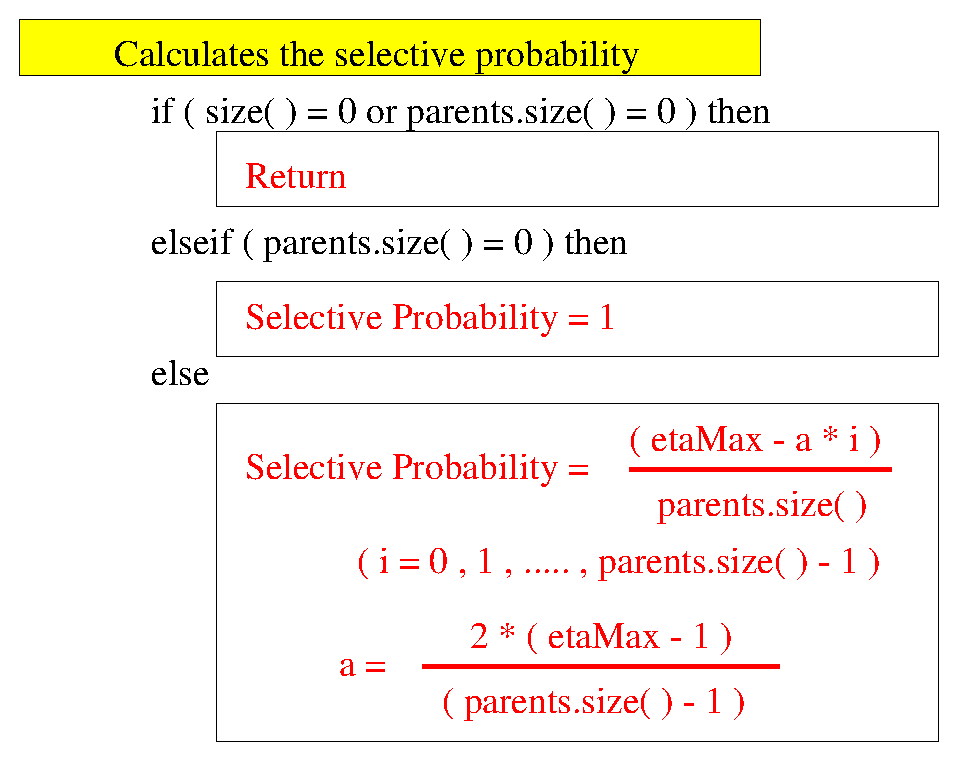
\includegraphics[width=7cm]{selectLinear1.eps}
\caption{Selective Probability}
\label{SelectLinear}
\end{center}
\end{figure}

\vspace*{2mm}

\noindent
\underline{parents.selectInit( );}

\noindent
We mentioned in {\em Select Individual 1}, internal variables {\em numCopies} and {\em
elitist} will be initialized. Please see the former explanation.

\begin{equation}
numCopies = 0
\end{equation}
\begin{equation}
elitist = false
\end{equation}

\vspace*{2mm}

\noindent
\underline{selectElitists( parents, numElitists );}

\noindent
{\em numElitists} individuals will be picked up as elitist(s). Please
see the former explanation.

\vspace*{2mm}

\noindent
\underline{selectRouletteWheel( parents, numElitists );}

\noindent
Using {\em selectElitists( parents, numElitists )}, {\em numElitists}
individuals were selected as elitist(s). These were stored in
(*this)[i] ( i = 0 , 1 , ... , numElitists - 1 ).

\noindent
After selecting elitists, the remaining individuals will be
selected by a roulette wheel. In order to select individuals,
selective probabilities and uniform random generators will be used. The
image of a roulette wheel is shown in Figure \ref{Roulette}.

\begin{figure}[h]
\begin{center}
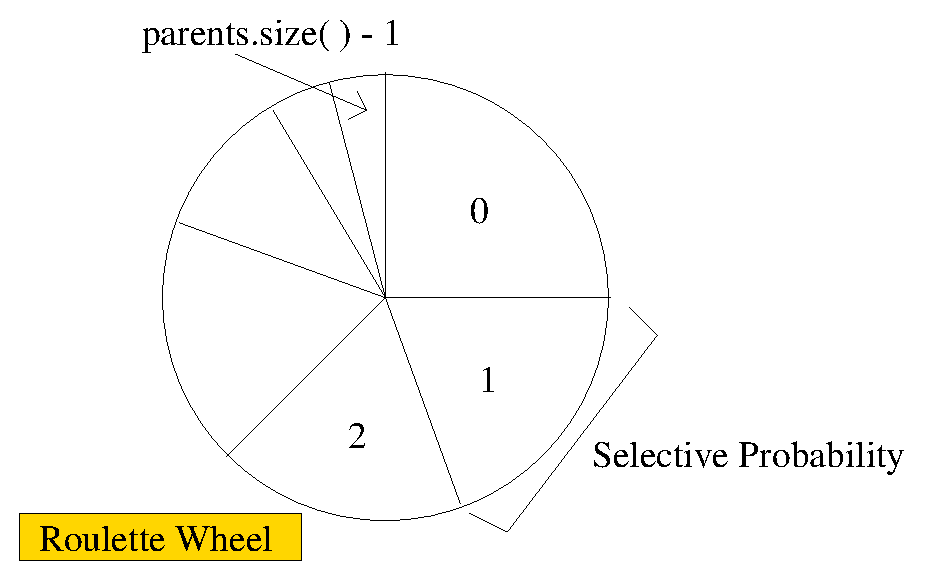
\includegraphics[width=6cm]{selectLinear2.eps}
\caption{Roulette Wheel}
\label{Roulette}
\end{center}
\end{figure}

\noindent
These will be stored in (*this)[i] ( i = numElitists , ... , parents.size(
) - 1 ).

\subsection{Generate Individual}

\noindent
In this section, we will explain the following function in {\em Class
Individual}. 

\begin{center}
Individual( const Chromosome\&, const Chromosome\& )
\end{center}

\noindent
The function prototype of this function was written in {\em
Individual.h} and the source code was written in {\em
Individual.cpp}. The function prototype and source code are given in Table
\ref{FP5} and Table \ref{SC5}

\begin{table}[h]
\begin{center}
\caption{The function prototype}
\label{FP5}
{\scriptsize
\begin{tabular}{|l|}\hline
\hspace*{7cm}\\
class Individual : private vector$<$ Chromosome * $>$\\
\{\\
\hspace*{4mm} public:\\
\hspace*{8mm} Individual( const Chromosome\&, \\
\hspace*{12mm} const Chromosome\& );\\
\}\\
\hspace*{7cm}\\\hline
\end{tabular}
}
\end{center}
\end{table}

\begin{table}[h]
\begin{center}
\caption{The source code}
\label{SC5}
{\scriptsize
\begin{tabular}{|l|}\hline
\hspace*{7cm}\\
Individual::Individual( const Chromosome\& chrom0, \\
\hspace*{4mm} const Chromosome\& chrom1 )\\
\hspace*{4mm} : vector$<$ Chromosome * $>$( 2 )\\
\{\\
\hspace*{4mm} *( begin( )) = chrom0.clone( );\\
\hspace*{4mm} *( begin( ) + 1 ) = chrom1.clone( );\\
\hspace*{4mm} fitness = 0;\\
\hspace*{4mm} scaledFitness = 0;\\
\hspace*{4mm} evalFlg = true;\\
\hspace*{4mm} feasible = 0;\\
\hspace*{4mm} selProb = 0.;\\
\hspace*{4mm} numCopies = 0;\\
\hspace*{4mm} elitist = false;\\
\hspace*{4mm} age = 0;\\
\}\\
\hspace*{7cm}\\\hline
\end{tabular}
}
\end{center}
\end{table}

\noindent
This function generates a new individual that consists of the
chromosomes {\em chrom0} and {\em chrom1}. In this function, internal
variables will be set as follows.

\begin{equation}
fitness = 0
\end{equation}
\begin{equation}
scaledFitness = 0
\end{equation}
\begin{equation}
evalFlg = true
\end{equation}
\begin{equation}
feasible = 0
\end{equation}
\begin{equation}
selProb = 0
\end{equation}
\begin{equation}
numCopies = 0
\end{equation}
\begin{equation}
elitist = false
\end{equation}
\begin{equation}
age = 0
\end{equation}

\noindent
Figure \ref{GenerateInd} gives the image of this function.

\begin{figure}[h]
\begin{center}
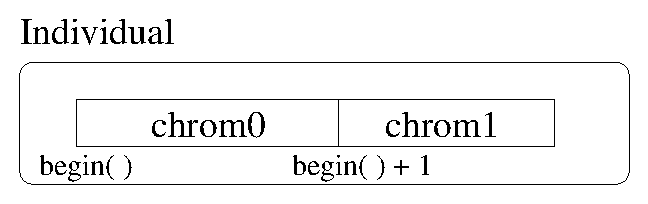
\includegraphics[width=5cm]{Individual.eps}
\caption{Generates a new individual}
\label{GenerateInd}
\end{center}
\end{figure}

\subsection{Crossover Chromosomes}

\noindent
In this section, we will explain the following function in {\em Class
ChromosomeT\_base}. 

\begin{center}
void crossoverUniform( const Chromosome\& dadChrom, const Chromosome\&
momChrom, const Chromosome\& posChrom )
\end{center}

\noindent
The source code of this function was written in {\em
ChromosomeT.h}. The source code is given in Table \ref{SC6}.

\begin{table}[h]
\begin{center}
\caption{The source code}
\label{SC6}
{\scriptsize
\begin{tabular}{|l|}\hline
\hspace*{7cm}\\
void crossoverUniform( const Chromosome\& dadChrom,\\
\hspace*{4mm} const Chromosome\& momChrom,\\
\hspace*{4mm} const Chromosome\& posChrom )\\
\{\\
\hspace*{4mm} crossoverUniform( dadChrom, momChrom,\\
\hspace*{8mm} dynamic\_cast$<$ const vector$<$ bool $>$\& $>$ \\
\hspace*{12mm} ( posChrom ) );\\
\}\\
\hspace*{7cm}\\\hline
\end{tabular}
}
\end{center}
\end{table}

\noindent
However, in order to undestand this function, we have to explain the
following function too.

\begin{center}
void crossoverUniform( const Chromosome\& dadChrom, const Chromosome\&
momChrom, const vector$<$ bool $>$\& pos )
\end{center}

\noindent
The source code is given in Table \ref{SC6-2}.

\begin{table}[h]
\begin{center}
\caption{The source code}
\label{SC6-2}
{\scriptsize
\begin{tabular}{|l|}\hline
\hspace*{7cm}\\
void crossoverUniform( const Chromosome\& dadChrom,\\
\hspace*{4mm} const Chromosome\& momChrom,\\
\hspace*{4mm} const vector$<$ bool $>$\& pos )\\
\{\\
\hspace*{4mm} SIZE\_CHECK( dadChrom.size( ) == \\
\hspace*{12mm} momChrom.size( ) )\\
\hspace*{4mm} resize( dadChrom.size( ) );\\
\hspace*{4mm} if( size( ) $>$ 0 ) \{\\
\hspace*{8mm} const vector$<$ T $>$\& dad = dynamic\_cast\\
\hspace*{12mm} $<$ const vector$<$ T $>$\& $>$( dadChrom );\\
\hspace*{8mm} const vector$<$ T $>$\& mom = dynamic\_cast\\
\hspace*{12mm} $<$ const vector$<$ T $>$\& $>$( momChrom );\\
\hspace*{8mm} for( unsigned i = min( size( ), pos.size( ) ); i--; )\\
\hspace*{12mm} ( *this )[ i ] = pos[ i ] ? mom[ i ] : dad[ i ];\\
\hspace*{4mm} \}\\
\}\\
\hspace*{7cm}\\\hline
\end{tabular}
}
\end{center}
\end{table}

\noindent
This function simulates crossover in chromosomes. The selected 
chromosomes are {\em dadChrom} and {\em momChrom}. Chromosome {\em
posChrom} and vector$<$ bool $>$ {\em pos} indicate which allele will be
used in {\em dadChrom} or {\em momChrom}.

\noindent
In the first function in Table \ref{SC6}, {\em Chromosome$\&$ posChrom} will
be cast to {\em const vector$<$ bool $>$$\&$} in order to use the next
function in Table \ref{SC6-2}.

\vspace*{2mm}

\noindent
\underline{SIZE\_CHECK( dadChrom.size( ) == }
\underline{momChrom.size( ) )}

\noindent
In this function, the size of the chromosome will be checked.

\vspace*{2mm}

\noindent
\underline{resize( dadChrom.size( ) )}

\noindent
In order to return values, (*this) will be adjusted to the size of {\em
dadChrom}.

\vspace*{2mm}

\noindent
\underline{if ( size( ) $>$ 0 \{ ..... \}}

\noindent
In this part, crossover will be done. At first, choromosomes {\em
dadChrom} and {\em momChrom} will be cast to {\em vector$<$ T $>$}. At
last, using the value of {\em pos[i]}, crossover will be done. If {\em
pos[i]} = true, the allele of {\em momChrom} will be copied and if false,
the allele of {\em dadChrom} will be copied.

\noindent
This image is given in Figure \ref{Crossover}.

\begin{figure}[h]
\begin{center}
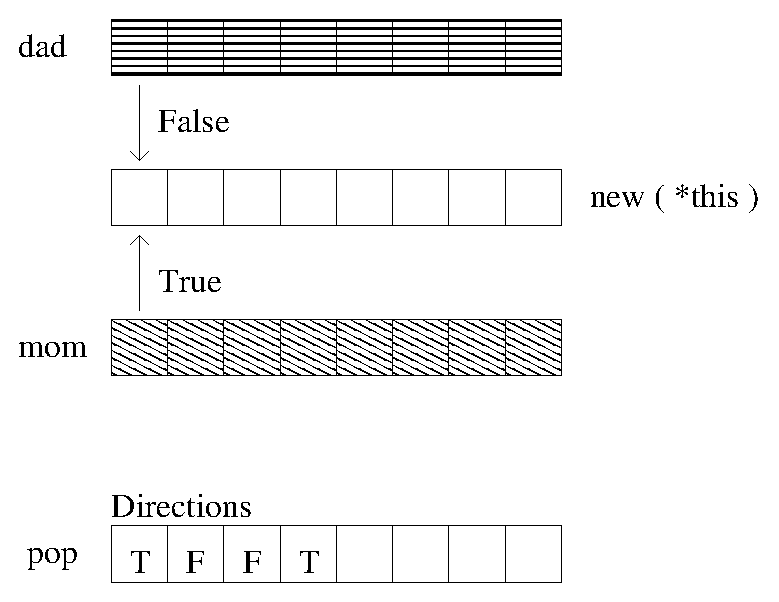
\includegraphics[width=6cm]{crossoveruniform.eps} 
\caption{Crossover Unifrom}
\label{Crossover}
\end{center}
\end{figure}

\subsection{Mutate Chromosome 1}

\noindent
In this section, we will explain the following function in {\em Class
ChromosomeT\_num}. 

\begin{center}
void mutateUniform( const Chromosome\& min, const Chromosome\& max,
const Chromosome\& p, bool cycle = false )
\end{center}

\noindent
The source code of this function was written in {\em
ChromosomeT.h}. The source code is given in Table \ref{SC7}.

\begin{table}[h]
\begin{center}
\caption{The source code}
\label{SC7}
{\scriptsize
\begin{tabular}{|l|}\hline
\hspace*{7cm}\\
void mutateUniform( const Chromosome\& min,\\
\hspace*{4mm} const Chromosome\& max,\\
\hspace*{4mm} const Chromosome\& p,  bool cycle = false )\\
\{\\
\hspace*{4mm} mutateUniform( min, max,\\
\hspace*{8mm} dynamic\_cast$<$ const vector$<$ double $>$\& $>$( p ),\\
\hspace*{8mm} cycle );\\
\}\\
\hspace*{7cm}\\\hline
\end{tabular}
}
\end{center}
\end{table}

\noindent
However, in order to undestand this function, we have to explain the
following function too.

\begin{center}
void mutateUniform( const Chromosome\& minChrom,\\
const Chromosome\& maxChrom,\\
const vector$<$ double $>$\& p, bool cycle = false )
\end{center}

\noindent
The source code is given in Table \ref{SC7-2}.

\begin{table}[h] 
\begin{center}
\caption{The source code}
\label{SC7-2}
{\scriptsize
\begin{tabular}{|l|}\hline
\hspace*{7cm}\\
void mutateUniform( const Chromosome\& minChrom,\\
\hspace*{4mm} const Chromosome\& maxChrom,\\
\hspace*{4mm} const vector$<$ double $>$\& p,\\
\hspace*{4mm} bool cycle = false )\\
\{\\
\hspace*{4mm} SIZE\_CHECK( size( ) == minChrom.size( ) )\\
\hspace*{4mm} SIZE\_CHECK( size( ) == maxChrom.size( ) )\\
\hspace*{4mm} RANGE\_CHECK( p.size( ) $<$= size( ) )\\
\hspace*{4mm} if( size( ) ) \{\\
\hspace*{8mm} const vector$<$ T $>$\& min = dynamic\_cast \\
\hspace*{12mm} $<$ const vector$<$ T $>$\& $>$( minChrom );\\
\hspace*{8mm} const vector$<$ T $>$\& max = dynamic\_cast \\
\hspace*{12mm} $<$ const vector$<$ T $>$\& $>$( maxChrom );\\
\hspace*{8mm} for( unsigned i = cycle ? size( ) : p.size( ); i--; )\\
\hspace*{12mm} if( Rng::coinToss( p[ i \% p.size( ) ] ) )\\
\hspace*{16mm} initialize( ( *this )[ i ], min[ i ], max[ i ] );\\
\hspace*{4mm} \}\\
\}\\
\hspace*{7cm}\\\hline
\end{tabular}
}
\end{center}
\end{table}

\noindent
This function simulates mutation in a chromosome. Mutation rates are
stored in {\em Chromosome$\&$ p} or {\em vector$<$ double $>$$\&$
p}. If mutation occurs, allele will be initialized in [ minChrom ,
maxChrom ]. If you see the {\em i}th allele, p[i], min[i] and max[i] will
be used to simulate mutation.

\noindent
In the first function in Table \ref{SC7}, {\em Chromosome$\&$ p} will be
cast to {\em const vector$<$ double $>$$\&$} in order to use the next
function in Table \ref{SC7-2}.

\vspace*{2mm}

\noindent
\underline{SIZE\_CHECK( size( ) == minChrom.size( ) )}

\noindent
\underline{SIZE\_CHECK( size( ) == maxChrom.size( ) )}

\noindent
At first, the size of minChrom, maxChrom and (*this) will be checked
in order to simulate mutation correctly.

\vspace*{2mm}

\noindent
\underline{RANGE\_CHECK( p.size( ) $<$ = size( )}

\noindent
Next, the size of p and (*this) will be checked. However, we can use
the values of p cyclically. Thus, the size of p should be less than or
equal to the size of (*this). Regarding the use of cyclic values, we will explain
later.

\vspace*{2mm}

\noindent
\underline{if ( size( ) )\{ ... \}}

\noindent
In this part, mutation will be done using coinToss trial. If
mutation occurs, (*this)[i] will be initialized in [ min[i] , max[i]
] like Figure \ref{MutateUniform}.

\begin{figure}[h]
\begin{center}
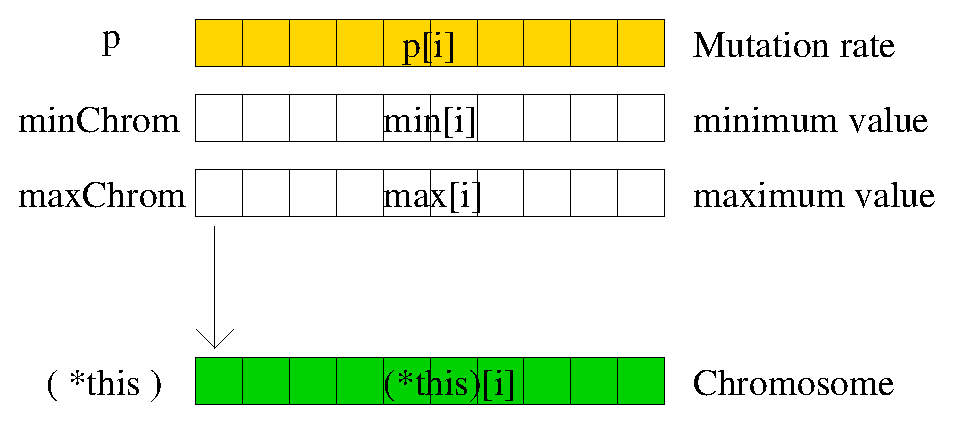
\includegraphics[width=6cm]{mutateUniform.eps}
\caption{Mutate Uniform}
\label{MutateUniform}
\end{center}
\end{figure}

\noindent
The image of cyclic use is given in Figure \ref{Cycle}. If cycle =
false, alleles from p.size( ) to size( )-1 will not be mutated at
all. If cycle = true, the mutation rate will be copied, see Figure
\ref{Cycle}.

\begin{figure}[h]
\begin{center}
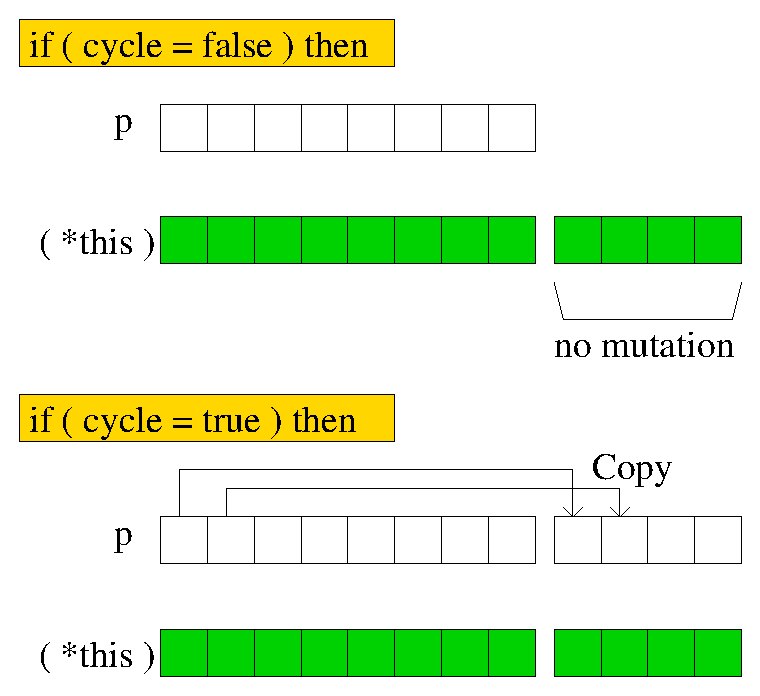
\includegraphics[width=5cm]{mutateUniform2.eps}
\caption{The image of cycle}
\label{Cycle}
\end{center}
\end{figure}

\subsection{Mutate Chromosome 2}

\noindent
In this section, we will explain the following function in {\em Class
ChromosomeT$<$ double $>$}. 

\begin{center}
void mutateNormal( const ChromosomeT$<$ double $>$\& stddev, bool =
false )
\end{center}

\noindent
The function prototype of this function was written in {\em
ChromosomeT.h} and the source code was written in {\em
ChromosomeT\_double.cpp}. The function prototype and source code are
given in Table \ref{FP8} and Table \ref{SC8}.

\begin{table}[h]
\begin{center}
\caption{The function prototype}
\label{FP8}
{\scriptsize
\begin{tabular}{|l|}\hline
\hspace*{7cm}\\
template $<$ $>$\\
class ChromosomeT$<$ double $>$ \\
\hspace*{4mm} : public ChromosomeT\_num$<$ double $>$\\
\{\\
\hspace*{4mm} public:\\
\hspace*{4mm} void mutateNormal( const ChromosomeT \\
\hspace*{8mm} $<$ double $>$\& stddev, bool = false );\\
\hspace*{7cm}\\\hline
\end{tabular}
}
\end{center}
\end{table}

\begin{table}[h]
\begin{center}
\caption{The source code}
\label{SC8}
{\scriptsize
\begin{tabular}{|l|}\hline
\hspace*{7cm}\\
void ChromosomeT$<$ double $>$::mutateNormal( \\
\hspace*{4mm} const Chromosome\& stdd, bool cycle )\\
\{\\
\hspace*{4mm} mutateNormal( dynamic\_cast \\
\hspace*{8mm} $<$ const vector$<$ double $>$\& $>$( stdd ), cycle );\\
\}\\
\hspace*{7cm}\\\hline
\end{tabular}
}
\end{center}
\end{table}

\noindent
However, in order to undestand this function, we have to explain the
following function too.

\begin{center}
void ChromosomeT$<$ double $>$::mutateNormal( const vector$<$ double
$>$\& stdd, bool cycle )
\end{center}

\noindent
The source code is given in Table \ref{SC8-2}.

\begin{table}[h] 
\begin{center}
\caption{The source code}
\label{SC8-2}
{\scriptsize
\begin{tabular}{|l|}\hline
\hspace*{7cm}\\
void ChromosomeT$<$ double $>$::mutateNormal( \\
\hspace*{4mm} const vector$<$ double $>$\& stdd,\\
\hspace*{4mm} bool cycle )\\
\{\\
\hspace*{4mm} RANGE\_CHECK( stdd.size( ) $<$= size( ) )\\
\hspace*{4mm} for( unsigned i = cycle ? size( ) : stdd.size( ); i--; )\\
\hspace*{8mm} ( *this )[ i ] += Rng::gauss( 0, \\
\hspace*{12mm} stdd[ i \% stdd.size( ) ] );\\
\}\\
\hspace*{7cm}\\\hline
\end{tabular}
}
\end{center}
\end{table}

\noindent
In the first function in Table \ref{SC8}, {\em Chromosome$\&$ stdd} will
be cast to {\em const vector$<$ double $>$$\&$} in order to use the
next function in Table \ref{SC8-2}.

\vspace{2mm}

\noindent
\underline{RANGE\_CHECK(stdd.size( ) $<$= size( ))}

\noindent
The size of stdd and (*this) will be checked. However, we can use the
values of stdd cyclically. Thus, the size of stdd should be less than
or equal to the size of (*this). We will show the use of cyclic values
in Figure \ref{MutateNormal}.

\vspace*{2mm}

\noindent
\underline{for( unsigned i = ... stdd.size( )]);}

\noindent
In this part, mutation will be done using the Gauss distribution. The
value {\em stdd( )} denotes the standard deviation. The mutation will
occur by the function {\em Rng::gauss(0,stdd[i\%stdd.size( )])}. This
image is shown in Figure \ref{MutateNormal}.

\vspace*{2mm}

\noindent
(*this)[i] means the {\em i}th allele. Using a standard deviation
stdd[i], the normal distribution will be calculated at first. After that,
this result will be added to (*this). This flow corresponds to the
following equation.

\begin{equation}
x(t) = x(t-1) + \tilde{z}
\end{equation}
\begin{equation}
\tilde{z} \sim N(0,\tilde{\sigma}(t))
\end{equation}

\begin{figure}[h]
\begin{center}
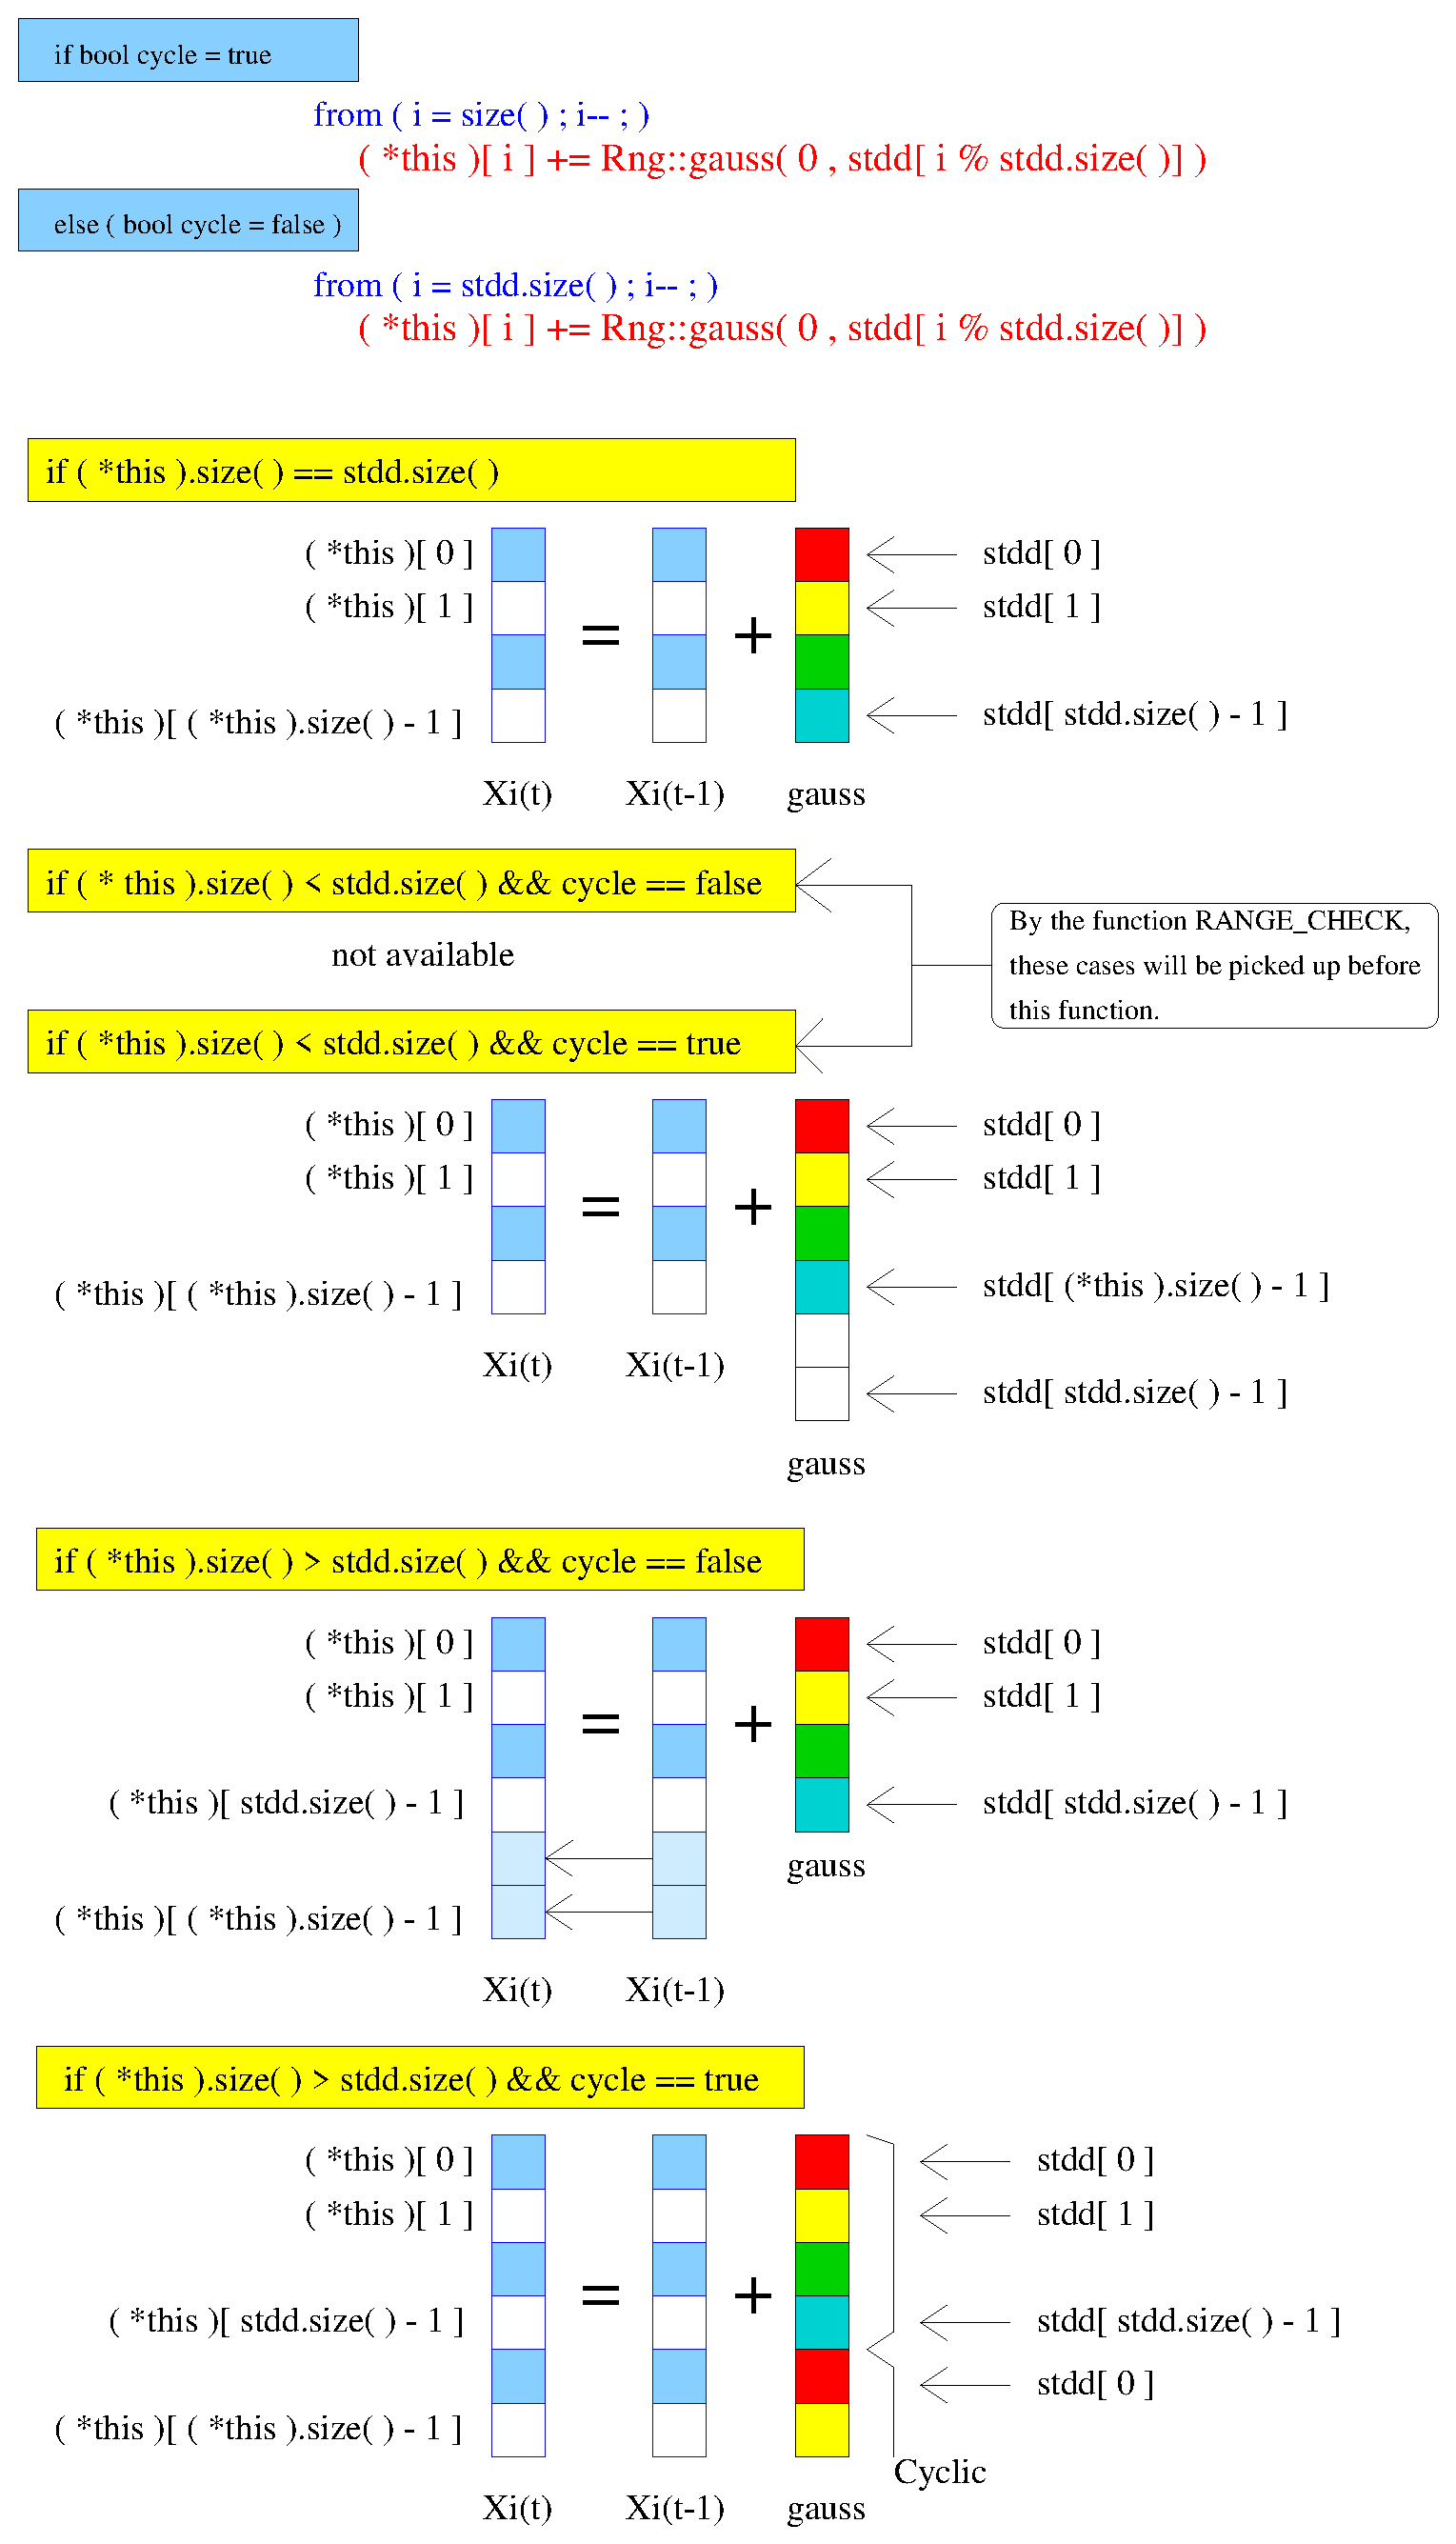
\includegraphics[width=8cm]{004-4-6-mutateNormal1.eps}
\caption{Mutate Normal}
\label{MutateNormal}
\end{center}
\end{figure}

\section{Recombine Chromosomes}

\noindent
In this section, we will explain the following function in {\em Class
ChromosomeT$<$ double $>$}. 

\begin{center}
void recombineIntermediate( Chromosome\& mate )
\end{center}

\noindent
The function prototype of this function was written in {\em
ChromosomeT.h} and the source code was written in {\em
ChromosomeT\_double.cpp}. The function prototype and source code are
given in Table \ref{FP9} and Table \ref{SC9}.

\begin{table}[h]
\begin{center}
\caption{The function prototype}
\label{FP9}
{\scriptsize
\begin{tabular}{|l|}\hline
\hspace*{7cm}\\
template $<$ $>$\\
class ChromosomeT$<$ double $>$ : \\
\hspace*{4mm} public ChromosomeT\_num$<$ double $>$\\
\{\\
\hspace*{4mm} public:\\
\hspace*{8mm} void recombineIntermediate( Chromosome\& );\\
\}\\
\hspace*{7cm}\\\hline
\end{tabular}
}
\end{center}
\end{table}

\begin{table}[h]
\begin{center}
\caption{The source code}
\label{SC9}
{\scriptsize
\begin{tabular}{|l|}\hline
\hspace*{7cm}\\
void ChromosomeT$<$ double $>$::recombineIntermediate( \\
\hspace*{4mm} Chromosome\& mate )\\
\{\\
\hspace*{4mm} SIZE\_CHECK( size( ) == mate.size( ) )\\
\hspace*{4mm} vector$<$ double $>$\& v = *this;\\
\hspace*{4mm} vector$<$ double $>$\& w = \\
\hspace*{4mm} dynamic\_cast$<$ vector$<$ double $>$\& $>$( mate );\\
\hspace*{4mm} for( unsigned i = v.size( ); i--; )\\
\hspace*{8mm} v[ i ] = w[ i ] = ( v[ i ] + w[ i ] ) / 2.;\\
\}\\
\hspace*{7cm}\\\hline
\end{tabular}
}
\end{center}
\end{table}

\noindent
This function simulates recombination in a chromosome. The allele in
the next generation will be the average between (*this) and {\em
mate}.

\vspace*{2mm}

\noindent
\underline{SIZE\_CHECK( size( ) == mate.size( ) )}

\noindent
At first, the size of (*this) and {\em mate} will be checked in order
to simulate recombination correctly.

\vspace*{2mm}

\noindent
\underline{vector$<$ double $>$\& v = *this;}

\noindent
\underline{vector$<$ double $>$\& w = }\\
\underline{dynamic\_cast$<$ vector $<$ double $>$\& $>$ ( mate );}

\noindent
The value of (*this) and {\em mate} will be stored in the vectors {\em
v} and {\em w}, respectively.

\vspace*{2mm}

\noindent
\underline{for( unsigned i ... ) ... /2.;}

\noindent
In this part, recombination will be done. The allele in the next
generation will be the average between {\em v} and {\em w}. The image
of this function is given in Figure \ref{Recombination}.

\begin{figure}[h]
\begin{center}
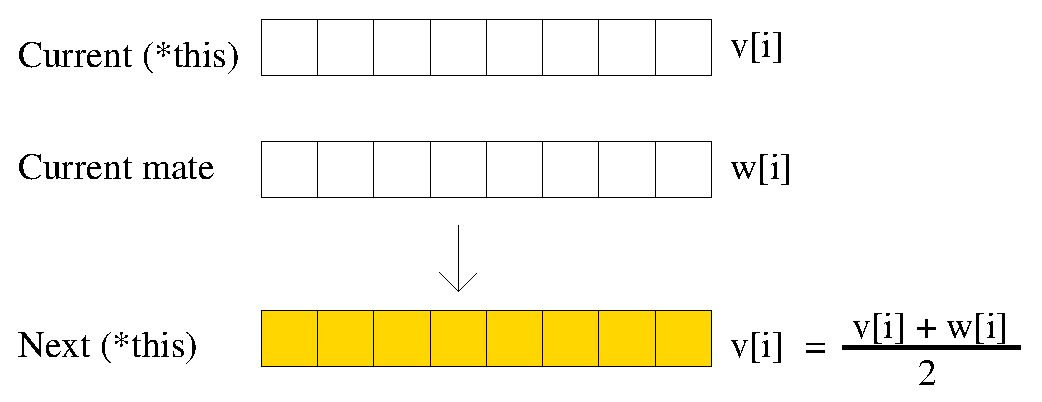
\includegraphics[width=6cm]{recombination.eps}
\caption{Recombination Intermediate}
\label{Recombination}
\end{center}
\end{figure}

%88888888888888888888888888888888888888888888888888888888888888888888
\section{Conclusions}

\noindent
In this report, we explained following topics.

\begin{enumerate}
\item Header files
\item Classes
\item Functions
\end{enumerate}

\noindent
We mentioned before, EALib has many classes and many functions. Thus, we
could not explain all. However, we believe that this internal report
will help you to understand the details of EALib.

\section*{Acknowledgement}

\noindent
The authors would like to thank Edger K\"{o}rner and Marc-Oliver Gewaltig for
their support.

%88888888888888888888888888888888888888888888888888888888888888888888
\begin{thebibliography}{99}

\bibitem{EALib-int-1997}
Martin Kreutz, Carsten Sievers, Axel W. Dietrich and Bernhard
Sendhoff, A  Programmers Guide to PAMPER - Classes \& Tools (P)arallel
(A)nd (M)odular (P)rogramming (E)nvi(r)onment, Internal Report of the
Institut f\"{u}r Neuroinformatik IRINI 97-03, 1997


\bibitem{EALib-Man-2000}
Martin Kreutz, Bernhard Sendhoff and Christian Igel, EALib : A C++
class library for evolutionary algorithms. Version 1.5, 2000.

\bibitem{EALib-Qui-2000}
R\"{u}diger Alberts, Quick Reference for the EA-Library, 2000.

\bibitem{EALib-Ref-2000}
R\"{u}diger Alberts, Reference for the EA-Library, 2000.

\bibitem{EALib-Address}
http://www.neuroinformatik.ruhr-uni-bochum.de/ini/PROJECTS/SONN
/Software/software.html.

\bibitem{GPL2}
http://www.gnu.org/licenses/gpl.html.


\end{thebibliography}

\clearpage

%88888888888888888888888888888888888888888888888888888888888888
%88   Appendix 888888888888888888888888888888888888888888888888
%88888888888888888888888888888888888888888888888888888888888888

\section*{Appendix A}

\noindent
The table \ref{AppA} shows other header files in EALib. The
declaration of {\em Population.h} does not include them. Thus,
in order to use them, please include the corresponding header file.

\newpage

\begin{table}[h]
\begin{center}
\caption{Other header files}
\label{AppA}
{\scriptsize
\begin{tabular}{|l|l|}\hline
Header file                &  The position                            \\\hline\hline
cma.h                      & */Shark-1.0/EALib/include/               \\\hline
arraY.h                    & */Shark-1.0/Tools/Array/include/         \\\hline
array.h                    & */Shark-1.0/Tools/Array/include/         \\\hline
arraycheck.h               & */Shark-1.0/Tools/Array/include/         \\\hline
arrayio.h                  & */Shark-1.0/Tools/Array/include/         \\\hline
arrayop.h                  & */Shark-1.0/Tools/Array/include/         \\\hline
arraysort.h                & */Shark-1.0/Tools/Array/include/         \\\hline
abs.h                      & */Shark-1.0/Tools/Basics/include/        \\\hline
cube.h                     & */Shark-1.0/Tools/Basics/include/        \\\hline
finite.h                   & */Shark-1.0/Tools/Basics/include/        \\\hline
Range.h                    & */Shark-1.0/Tools/Basics/include/        \\\hline
sign.h                     & */Shark-1.0/Tools/Basics/include/        \\\hline
sqr.h                      & */Shark-1.0/Tools/Basics/include/        \\\hline
FileUtil.h                 & */Shark-1.0/Tools/FileUtil/include/      \\\hline
arraylinalg.h              & */Shark-1.0/Tools/LinAlg/include/        \\\hline
arrayoptimize.h            & */Shark-1.0/Tools/LinAlg/include/        \\\hline
klt.h                      & */Shark-1.0/Tools/LinAlg/include/        \\\hline
linalg.h                   & */Shark-1.0/Tools/LinAlg/include/        \\\hline
lr.h                       & */Shark-1.0/Tools/LinAlg/include/        \\\hline
MathExt.h                  & */Shark-1.0/Tools/Math/include/          \\\hline
Metric.h                   & */Shark-1.0/Tools/Metric/include/        \\\hline
Binomial.h                 & */Shark-1.0/Tools/Rng/include/           \\\hline
Erlang.h                   & */Shark-1.0/Tools/Rng/include/           \\\hline
HyperGeometric.h           & */Shark-1.0/Tools/Rng/include/           \\\hline
LogNormal.h                & */Shark-1.0/Tools/Rng/include/           \\\hline
NegExponential.h           & */Shark-1.0/Tools/Rng/include/           \\\hline
Weibull.h                  & */Shark-1.0/Tools/Rng/include/           \\\hline
CodeBook.h                 & */Shark-1.0/Mixture/include/             \\\hline
KernelDensity.h            & */Shark-1.0/Mixture/include/             \\\hline
LinearRegression.h         & */Shark-1.0/Mixture/include/             \\\hline
LocalLinear                & */Shark-1.0/Mixture/include/             \\
\hspace*{2mm} Regression.h &                                          \\\hline
MixtureModel.h             & */Shark-1.0/Mixture/include/             \\\hline
MixtureOf                  & */Shark-1.0/Mixture/include/             \\
\hspace*{2mm} Gaussians.h  &                                          \\\hline  
PCA.h                      & */Shark-1.0/Mixture/include/             \\\hline
RandomVector.h             & */Shark-1.0/Mixture/include/             \\\hline
RBFN-PTO.h                 & */Shark-1.0/Mixture/include/             \\\hline
RBFN.h                     & */Shark-1.0/Mixture/include/             \\\hline
Ring.h                     & */Shark-1.0/TestData/RandomDistr         \\
                           & \hspace{2mm} /include                    \\\hline
BimodalBrownian            & */Shark-1.0/TestData                     \\
\hspace*{2mm} Process.h    & \hspace{2mm} /TimeSeries/include         \\\hline
Counter.h                  & */Shark-1.0/TestData                     \\
                           & \hspace{2mm} /TimeSeries/include         \\\hline
DiscreteMackey             & */Shark-1.0/TestData                     \\
\hspace*{2mm} Glass.h      & \hspace{2mm} /TimeSeries/include         \\\hline
Embedding.h                & */Shark-1.0/TestData                     \\
                           & \hspace{2mm} /TimeSeries/include         \\\hline
Generator.h                & */Shark-1.0/TestData                     \\
                           & \hspace{2mm} /TimeSeries/include         \\\hline
IOGenerator.h              & */Shark-1.0/TestData                     \\
                           & \hspace{2mm} /TimeSeries/include         \\\hline
IOSamples.h                & */Shark-1.0/TestData                     \\
                           & \hspace{2mm} /TimeSeries/include         \\\hline
Lorenz63.h                 & */Shark-1.0/TestData                     \\
                           & \hspace{2mm} /TimeSeries/include         \\\hline
Lorenz84.h                 & */Shark-1.0/TestData                     \\
                           & \hspace{2mm} /TimeSeries/include         \\\hline
MackeyGlass.h              & */Shark-1.0/TestData                     \\
                           & \hspace{2mm} /TimeSeries/include         \\\hline
NoisyIO                    & */Shark-1.0/TestData                     \\
\hspace*{2mm} Samples.h    & \hspace{2mm} /TimeSeries/include         \\\hline
NoisyMackey                & */Shark-1.0/TestData                     \\
\hspace*{2mm} Glass.h      & \hspace{2mm} /TimeSeries/include         \\\hline
RK4-1D.h                   & */Shark-1.0/TestData                     \\
                           & \hspace{2mm} /TimeSeries/include         \\\hline
RK4.h                      & */Shark-1.0/TestData                     \\
                           & \hspace{2mm} /TimeSeries/include         \\\hline
SelectComponent.h          & */Shark-1.0/TestData                     \\
                           & \hspace{2mm} /TimeSeries/include         \\\hline
\end{tabular}
}
\end{center}
\end{table}

\clearpage

\section*{Appendix B}

\noindent
In Table \ref{AppB}, we will show many other classes. We can not use these
classes without a special declaration,  because the corresponding header
files are not included by {\em Population.h}!

\newpage

\begin{table}[h]
\begin{center}
\caption{Other classes}
\label{AppB}
{\scriptsize
\begin{tabular}{|l|l|}\hline
File name \hspace{10mm}      & Including classes \hspace{15mm}       \\\hline\hline 
cma.h                        & $Class \ CMA                        $ \\\hline
arraY.h                      & $Class \ arraY                      $ \\\hline
array.h                      & $Class \ arraybase                  $ \\
                             & $Class \ array                      $ \\
                             & $Class \ array\_reference           $ \\\hline
arraycheck.h                 & $Class \ check\_exception           $ \\\hline
arrayio.h                    & ( nothing )                           \\\hline
arrayop.h                    & ( nothing )                           \\\hline
arraysort.h                  & ( nothing )                           \\\hline
abs.h                        & ( nothing )                           \\\hline
cube.h                       & ( nothing )                           \\\hline
finite.h                     & ( nothing )                           \\\hline
Range.h                      & $Class \ Range                      $ \\\hline
sign.h                       & ( nothing )                           \\\hline
sqr.h                        & ( nothing )                           \\\hline
FileUtil.h                   & ( nothing )                           \\\hline
arraylinalg.h                & ( nothing )                           \\\hline
arrayoptimize.h              & ( nothing )                           \\\hline
klt.h                        & ( nothing )                           \\\hline
linalg.h                     & ( nothing )                           \\\hline
lr.h                         & ( nothing )                           \\\hline
MathExt.h                    & ( nothing )                           \\\hline
Metric.h                     & $Class \ Metric                     $ \\\hline
Binomial.h                   & $Class \ Binomial                   $ \\\hline
Erlang.h                     & $Class \ Erlang                     $ \\\hline
HyperGeometric.h             & $Class \ HyperGeometric             $ \\\hline
LogNormal.h                  & $Class \ LogNormal                  $ \\\hline
NegExponential.h             & $Class \ NegExponential             $ \\\hline
Weibull.h                    & $Class \ Weibull                    $ \\\hline
CodeBook.h                   & $Class \ CodeBook                   $ \\\hline
KernelDensity.h              & $Class \ KernelDensity              $ \\\hline
LinearRegression.h           & $Class \ LinearRegression           $ \\\hline
LocalLinearRegression.h      & $Class \ LocalLinearRegression      $ \\\hline
MixtureModel.h               & $Class \ MixtureModel               $ \\\hline
MixtureOfGaussians.h         & $Class \ MixtureOfGaussians         $ \\\hline
PCA.h                        & $Class \ PCA                        $ \\\hline
RandomVector.h               & $Class \ RandomVector               $ \\\hline
RBFN-PTO.h                   & $Class \ RBFN\_PTO                  $ \\\hline
RBFN.h                       & $Class \ RBFN                       $ \\\hline
Ring.h                       & $Class \ Ring                       $ \\\hline
BimodalBrownian              & $Class \ BimodalBrownian            $ \\
\hspace*{2mm} Process.h      & \hspace{2mm} $ Process              $ \\\hline
Counter.h                    & $Class \ Counter                    $ \\\hline
DiscreteMackeyGlass.h        & $Class \ DiscreteMackeyGlass        $ \\\hline
Embedding.h                  & $Class \ Embedding                  $ \\\hline
Generator.h                  & $Class \ Generator                  $ \\\hline
IOGenerator.h                & $Class \ IOGenerator                $ \\\hline
IOSamples.h                  & $Class \ IOSamples                  $ \\\hline
Lorenz63.h                   & $Class \ Lorenz63                   $ \\\hline
Lorenz84.h                   & $Class \ Lorenz84                   $ \\\hline
MackeyGlass.h                & $Class \ MackeyGlass                $ \\\hline
NoisyIOSamples.h             & $Class \ NoisyIOSamples             $ \\\hline
NoisyMackeyGlass.h           & $Class \ NoisyMackeyGlass           $ \\\hline
RK4-1D.h                     & $Class \ RK4\_1D                    $ \\\hline
RK4.h                        & $Class \ RK4                        $ \\\hline
SelectComponent.h            & $Class \ SelectComponent            $ \\\hline
\end{tabular}
}
\end{center}
\end{table}

\clearpage

\section*{Appendix C}

\noindent
Table \ref{AppC} shows the number of functions in each class. These
include virtual functions, friend functions and inline functions.

\newpage

\vspace*{20mm}

\begin{table}[h]
\begin{center}
\caption{The number of other functions}
\label{AppC}
\vspace*{5mm}
{\scriptsize
\begin{tabular}{|l|l|l|l|l|}\hline
Name of Class                 & Public & Private & Protect & Others  \\\hline\hline
$CMA                        $ &     18 &       0 &       0 &       0 \\\hline
$arraY                      $ &     10 &       0 &       0 &       0 \\\hline
$arraybase                  $ &     11 &       0 &       2 &       8 \\\hline
$array                      $ &     74 &       0 &       4 &       0 \\\hline
$array\_reference           $ &      7 &       0 &       0 &       0 \\\hline
$check\_exception           $ &      2 &       0 &       0 &       0 \\\hline
$Range                      $ &      8 &       0 &       0 &       0 \\\hline
$Metric                     $ &      8 &       0 &       0 &       0 \\\hline
$Binomial                   $ &      7 &       0 &       0 &       0 \\\hline
$Erlang                     $ &      9 &       1 &       0 &       0 \\\hline
$HyperGeometric             $ &      8 &       1 &       0 &       0 \\\hline
$LogNormal                  $ &      8 &       1 &       0 &       0 \\\hline
$NegExponential             $ &      7 &       0 &       0 &       0 \\\hline
$Weibull                    $ &      9 &       0 &       0 &       0 \\\hline
$CodeBook                   $ &     10 &       0 &       0 &       0 \\\hline
$KernelDensity              $ &      6 &       0 &       1 &       0 \\\hline
$LinearRegression           $ &     11 &       0 &       0 &       0 \\\hline
$LocalLinear                $ &      8 &       1 &       0 &       0 \\
\hspace*{2mm} $Regression   $ &        &         &         &         \\\hline   
$MixtureModel               $ &     11 &       0 &       2 &       4 \\\hline
$MixtureOf                  $ &    104 &       0 &       3 &       3 \\
\hspace*{2mm} $Gaussians    $ &        &         &         &         \\\hline
$PCA                        $ &     11 &       0 &       0 &       0 \\\hline
$RandomVector               $ &      1 &       0 &       1 &       0 \\\hline
$RBFN\_PTO                  $ &      2 &       6 &       0 &       0 \\\hline
$RBFN                       $ &     26 &       0 &       3 &       1 \\\hline
$Ring                       $ &     12 &       2 &       0 &       0 \\\hline
$BimodalBrownian            $ &      2 &       2 &       0 &       0 \\
\hspace*{2mm} $Process      $ &        &         &         &         \\\hline
$Counter                    $ &      3 &       1 &       0 &       0 \\\hline
$DiscreteMackey             $ &      3 &       1 &       0 &       0 \\
\hspace*{2mm} $Glass        $ &        &         &         &         \\\hline
$Embedding                  $ &     12 &       0 &       1 &       0 \\\hline
$Generator                  $ &      0 &       0 &       0 &       4 \\\hline
$IOGenerator                $ &      0 &       0 &       0 &       4 \\\hline
$IOSamples                  $ &     11 &       0 &       1 &       0 \\\hline
$Lorenz63                   $ &      1 &       2 &       0 &       0 \\\hline
$Lorenz84                   $ &      1 &       2 &       0 &       0 \\\hline
$MackeyGlass                $ &      3 &       2 &       0 &       0 \\\hline
$NoisyIOSamples             $ &      9 &       0 &       1 &       0 \\\hline
$NoisyMackeyGlass           $ &      6 &       1 &       0 &       0 \\\hline
$RK4\_1D                    $ &      3 &       0 &       0 &       1 \\\hline
$RK4                        $ &      3 &       0 &       0 &       1 \\\hline
$SelectComponent            $ &      5 &       1 &       0 &       0 \\\hline
\end{tabular}
}
\end{center}
\end{table}








\end{document}